\documentclass[10pt,journal,cspaper,compsoc]{IEEEtran}

\usepackage{graphicx}
\usepackage{amsmath}
\usepackage{amssymb}
\usepackage{amsbsy}
\usepackage{xfrac}
\usepackage{subcaption}
\usepackage{algorithm}
\usepackage{algpseudocode}

\usepackage[breaklinks=true,bookmarks=false]{hyperref}

\newcommand{\abs}[1]{\lvert #1 \rvert}
\newcommand{\norm}[1]{\lVert #1 \rVert}
\newcommand{\sgn}{\operatorname{sgn}}
\newcommand{\argmin}{\operatorname{arg\!min}}
\newcommand{\argmax}{\operatorname{arg\!max}}
\newcommand{\R}{\mathbb{R}}
\newcommand{\hilbert}{\mathcal{H}}

% Inner product mapping
\newcommand{\ip}{\phi_{IP}(\boldsymbol{x}_k)}
% Inverse inner product mapping
\newcommand{\invip}{{\phi_{IP}}^{-1}(\boldsymbol{v}_k)}
% Spherical mapping
\newcommand{\spher}{\phi_{SPHER}(\boldsymbol{x}_k)}
% Inverse Spherical mapping
\newcommand{\invspher}{{\phi_{SPHER}}^{-1}(\boldsymbol{v}_k)}
% AEP mapping
\newcommand{\aep}{\phi_{AEP}(\boldsymbol{x}_k)}
% Inverse AEP mapping
\newcommand{\invaep}{{\phi_{AEP}}^{-1}(\boldsymbol{v}_k)}
% PGA mapping
\newcommand{\pga}{\phi_{PGA}(\boldsymbol{x}_k)}
% Inverse PGA mapping
\newcommand{\invpga}{{\phi_{PGA}}^{-1}(\boldsymbol{v}_k)}
% Least squares mapping
\newcommand{\ls}{\phi_{LS}(\boldsymbol{x}_k)}
% Inverse least squares mapping
\newcommand{\invls}{{\phi_{LS}}^{-1}(\boldsymbol{v}_k)}


% Image commands
\newcommand{\origimg}[1]{
    \begin{subfigure}{0.11\textwidth}
            \centering
            \includegraphics[width=\textwidth]{images/results/photoface/#1.png}
            \label{fig:results-photoface-input-#1}
    \end{subfigure}
}
\newcommand{\origimgtop}[2]{
    \begin{subfigure}{0.11\textwidth}
            \centering
            \caption*{#2}
            \includegraphics[width=\textwidth]{images/results/photoface/#1.png}
            \label{fig:results-photoface-input-#1}
    \end{subfigure}
}
\newcommand{\sfsimgs}[2]{
    \begin{subfigure}{0.11\textwidth}
            \centering
            \includegraphics[width=\textwidth]{images/results/photoface/#1_#2.png}
            \label{fig:results-photoface-#1-#2}
    \end{subfigure}
}
\newcommand{\sfsimgstop}[3]{
    \begin{subfigure}{0.11\textwidth}
            \centering
            \caption*{#2}
            \includegraphics[width=\textwidth]{images/results/photoface/#1_#3.png}
            \label{fig:results-photoface-#1-#3}
    \end{subfigure}
}

\newcommand{\sfsimgsalltop}[1]{
    \origimgtop{#1}{Input Image}
    \sfsimgstop{#1}{Ground Truth}{ground_truth}
    \sfsimgstop{#1}{AEP}{aep}
    \sfsimgstop{#1}{IP}{cosine}
    \sfsimgstop{#1}{PGA}{pga}
    \sfsimgstop{#1}{SPHERICAL}{spherical}
    \sfsimgstop{#1}{SIRFS}{sirfs}
}

\newcommand{\sfsimgsall}[1]{
    \origimg{#1}
    \sfsimgs{#1}{ground_truth}
    \sfsimgs{#1}{aep}
    \sfsimgs{#1}{cosine}
    \sfsimgs{#1}{pga}
    \sfsimgs{#1}{spherical}
    \sfsimgs{#1}{sirfs}
} % Load commands

\begin{document}

\title{Lucas-Kanade on Normals}


\author{Patrick~Snape,~\IEEEmembership{Student~Member,~IEEE,}
        and~Stefanos~Zafeiriou,~\IEEEmembership{Member,~IEEE}}


% The paper headers
%\markboth{IEEE Transactions On Pattern Analysis And Machine Intelligence,~Vol.~1, No.~1, December~2013}{A}


\IEEEcompsoctitleabstractindextext{%
\begin{abstract}
The unwritten abstract.
\end{abstract}

\begin{keywords}
Normals, Active Appearance Models, Shape-From-Shading
\end{keywords}}


\maketitle


% To allow for easy dual compilation without having to reenter the
% abstract/keywords data, the \IEEEcompsoctitleabstractindextext text will
% not be used in maketitle, but will appear (i.e., to be "transported")
% here as \IEEEdisplaynotcompsoctitleabstractindextext when compsoc mode
% is not selected <OR> if conference mode is selected - because compsoc
% conference papers position the abstract like regular (non-compsoc)
% papers do!
\IEEEdisplaynotcompsoctitleabstractindextext
% For peerreview papers, this IEEEtran command inserts a page break and
% creates the second title. It will be ignored for other modes.
\IEEEpeerreviewmaketitle

%\ifCLASSOPTIONcompsoc
%  \noindent\raisebox{2\baselineskip}[0pt][0pt]%
%  {\parbox{\columnwidth}{\section{Introduction}\label{sec:introduction}%
%  \global\everypar=\everypar}}%
%  \vspace{-1\baselineskip}\vspace{-\parskip}\par
%\else
%  \section{Introduction}\label{sec:introduction}\par
%\fi
%
% Admittedly, this is a hack and may well be fragile, but seems to do the
% trick for me. Note the need to keep any \label that may be used right
% after \section in the above as the hack puts \section within a raised box.



% The very first letter is a 2 line initial drop letter followed
% by the rest of the first word in caps (small caps for compsoc).
% 
% form to use if the first word consists of a single letter:
% \IEEEPARstart{A}{demo} file is ....
% 
% form to use if you need the single drop letter followed by
% normal text (unknown if ever used by IEEE):
% \IEEEPARstart{A}{}demo file is ....
% 
% Some journals put the first two words in caps:
% \IEEEPARstart{T}{his demo} file is ....
% 
% Here we have the typical use of a "T" for an initial drop letter
% and "HIS" in caps to complete the first word.

% use section* for acknowledgement
%\ifCLASSOPTIONcompsoc
  % The Computer Society usually uses the plural form
%  \section*{Acknowledgments}
%\else
  % regular IEEE prefers the singular form
%  \section*{Acknowledgment}
%\fi

%Acknowledgment text

\section{Introduction}\label{sec:introduction}
\IEEEPARstart{S}{ince} Lucas and Kanade first proposed their optical-flow algorithm \cite{RefWorks:71}, it has become the de facto choice for image alignment. Today, LK does not represent a single algorithm, but rather a broad family of algorithms. These algorithms can be categorised as seeking to minimise a given cost function by optimising over a parametrised warp function. Many different approaches have been proposed to solve the original LK algorithm, but by far the most popular is the inverse compositional (IC) update proposed by Baker and Matthews \cite{RefWorks:10}. In \cite{RefWorks:10}, Baker and Matthews show that the IC update gives a very computationally efficient method of solving the $\ltwo$ norm minimisation. 

Although efficient, the sum of squared deviations (SSD) used in the IC update is not robust. Therefore, more recent work has concentrated on robustness to outliers such as occlusions and variable illumination. These attempts fall roughly in to two major categories: replacing the SSD with a robust objective function \cite{RefWorks:59, RefWorks:72, RefWorks:53, RefWorks:274} or replacing pixel intensities with a more informative feature space \cite{RefWorks:73, RefWorks:6, RefWorks:273}. For example, Evangelidis and Psarakis \cite{RefWorks:59} replace the SSD with the Enhanced Correlation Coefficient (ECC) which seeks to minimise over the normalised pixel intensities. They provide an IC update of the ECC cost function and prove its invariance to illumination changes. Illumination invariance was also shown by Dowsen and Bowden in \cite{RefWorks:72}. Here, they propose a mutual information based cost function and, with additional assumptions, also give a computationally efficient algorithm. 

Lucey et al. \cite{RefWorks:67, RefWorks:73} showed that SSD measures can be robust if performed on features other than pixel intensities. In particular, they formulate the LK algorithm within the 2D Fourier domain and show that image alignment on banks of filter responses is equivalent to a weighted alignment of pixel intensities. Cootes and Taylor \cite{RefWorks:273} use local image features in the form of edge orientations in order to exploit the underlying object structure.

Although the Lucas-Kanade (LK) algorithm describes a gradient descent methodology for aligning arbitrary objects, much of the literature concentrates on its use in facial alignment. This is due, in part, to the large number of facial images available for study, as well as interesting uses of facial analysis in security, medicine and entertainment. More recently, cheap consumer hardware, such as the Microsoft Kinect, has seen increased availability of depth images of faces. Depth images have the advantage of being a more descriptive medium than pixel intensities, as they are insensitive to illumination and give an explicit representation of shape. The previously discussed LK algorithms, whilst robust for intensity images, do not make use of this more powerful representation. In particular, they focus on insensitivity to illumination variation, which is not an issue for depth data. However, depth data suffers from its own issues, most notably lack of spatial accuracy and noise. For this reason, we propose a robust feature space for depth data, which comes in the form of normals.

Normals, in depth images, are defined as the vectors that lie perpendicular to the object surface at a given point. A depth image can be seen as a surface with a triangulation that is given implicitly by its discrete gridded nature. Each pixel is a member of multiple triangles and a normal can be calculated per-triangle. Therefore, the per-pixel normal is defined as the mean of the per-triangle normals that the pixel is a member of. Normals are most commonly investigated in conjunction with depth recovery techniques such as Shape-From-Shading (SFS) \cite{RefWorks:249, RefWorks:252, RefWorks:270, RefWorks:225} and photometric stereo \cite{RefWorks:268, RefWorks:108}. Shape-From-X techniques, including SFS, seek to recover shape from images by using different cues within an image. In the case of SFS, shape is recovered from a single image, under a single point light source, by assuming the object to be smooth and exhibit lambertian reflectance. However, SFS is, in general, an ill-defined problem. To overcome this, Smith and Hancock \cite{RefWorks:86, RefWorks:90} proposed a statistical prior on normals in facial images that produces accurate results with low-computational overhead. Their major contribution, however, was in noting that linear statistical analysis cannot be applied directly to normals. This is due to the fact that distances between normals are non-linear, and are actually best described as paths along the surface of a unit sphere. Smith and Hancock propose two separate methodologies for performing statistical analysis on normals. In \cite{RefWorks:90} they propose the Azimuthal Equidistant Projection (AEP), which projects normals on to their local tangent plane and allows for linear analysis in the tangent space. In \cite{RefWorks:86}, they extend the Principal Geodesic Analysis (PGA) proposed by Fletcher et al. \cite{RefWorks:100} to the domain of normals.

Unfortunately, even robust image alignment algorithms are not capable of handling large variations in appearance. In faces, these variations include pose, gender and identity. For this reason, Active Appearance Models (AAMs) were proposed \cite{RefWorks:95,RefWorks:227}. AAMs extend the LK algorithm to include statistical priors on appearance and shape and allow for complex object alignment. AAMs focus on modelling appearance variation according to a set of linear basis that is learnt offline. In the case of faces, the appearance model is able to represent changes in pose and identity. However, the canonical AAM as described by \cite{RefWorks:95} uses an SSD objective function and thus is not robust to outliers. In depth data, these outliers include occlusions and the noise within the data.

3D Morphable Models (3DMM) \cite{RefWorks:96}, represent the state-of-the-art for statistical fitting algorithms. 3DMMs combine a more complex model of appearance, shape and lighting than AAMs, and thus are more accurate at the expense of being less efficient. Even the more efficient inverse alignment method of \cite{RefWorks:275} is not able to match the real-time capabilities of AAMs \cite{RefWorks:233, RefWorks:236}. Many attempts have been made to recover 3D shape using AAMs \cite{RefWorks:233, RefWorks:236, RefWorks:258, RefWorks:257}. These attempts involve using a 3D shape prior in order to infer the depth from the sparse landmarks. Given that depth images already encode all three-dimensions, it is not necessary to couple our AAM with a 3D sparse shape model. Fanelli et al. \cite{RefWorks:236}, inspired by \cite{RefWorks:276}, used a random forest based approach to provide real-time fitting using depth images. However, due to the cascade of regressors used, their method requires training on far more images than a simple gradient descent based AAM such as ours.

In this work we are interested in robust facial alignment in depth images. We seek to align faces with changing identity and pose, which is possible through the use of algorithms such as AAMs. However, we wish to perform the alignment on noisy data with very little pre-processing. To achieve this, we propose the use of normals to minimise the effect of outliers. The use of normals as a robust subspace is motivated by previous work on using orientations for object alignment \cite{RefWorks:273, RefWorks:6, RefWorks:272}. Since normals encode the orientation of a surface, we can exploit previous work on the robustness of orientation features. For example, Tzimiropoulos et al. \cite{RefWorks:5} have shown that the cosine of orientations represent a theoretically robust subspace for linear analysis. By providing an angular representation of normals, we show that normals also exhibit a theoretically robust subspace.

In order to use normals as an appearance space within AAMs, we need to be able to perform statistical analysis on normals. Therefore, we present a kernel-based framework for non-linear analysis of normals. Due to the generality of our kernel-based framework, we also present results within the SFS framework of \cite{RefWorks:90}.

Summarising, our key contributions are:
%%%%%%%%%%%%%%%%%%%%%%%%%%
\begin{itemize}
  \item We use the insight given by the theoretical robustness of the cosine correlation and propose a novel cost function for the LK algorithm based on the cosine of the angle between normals.
  \item We provide a kernel-based framework for performing statistical component analysis of normals. We formulate two existing projection operations, the Azimuthal Equidistant Projection \cite{RefWorks:90} and Principal Geodesic Analysis \cite{RefWorks:86} within this framework.
  \item We provide a novel robust kernel based on the cosine of the angles between normals. We also show that components can be extracted directly from normals, which becomes clear within the kernel framework.
  \item Finally, we use our kernel framework to provide a robust AAM for facial depth images and show it's substantial performance improvement over raw depth data.
\end{itemize}
%%%%%%%%%%%%%%%%%%%%%%%%%%
\subsection{Notation of Normals}\label{subsec:notation-normals}
We are interested in image-based alignment and analysis and so assume that we are dealing with needle-maps. A needle-map describes a surface $z(i, j)$ in terms of the normal $\boldsymbol{n}(i, j) = [x_{ij}, y_{ij}, z_{ij}]^T$, aligned such that all normals point towards the camera plane. In the case of a set of training images, as used in statistical analysis, we denote the vector of normals of length $N$, for image $k$, as $\boldsymbol{x}_k = (x_k^1, y_k^1, z_k^1, \ldots, x_k^N, y_k^N, z_k^N)^T$.
%%%%%%%%%%%%%%%%%%%%%%%%%%
\subsection{Notation of LK}\label{subsec:notation-lk}
When referring to the operations performed by the LK algorithm we will use the following notations, borrowed from \cite{RefWorks:67}. Vectors are always presented in lower case bold, as in normals ($\boldsymbol{n}$), matrices are in upper case bold ($\boldsymbol{X}$) and scalars in lower case ($x$). Images are denoted in capitalised form as in $I$. Warp functions $\mathcal{W}(\boldsymbol{x}_i;\p) = \left[ \mathcal{W}_x(\boldsymbol{x}_i;\p), \mathcal{W}_y(\boldsymbol{x}_i;\p) \right]$ express the warping of the $i$th 2D coordinate vector $\boldsymbol{x}_i = [x_i, y_i]^T$ by a set of parameters $\p = \left[p(1), ..., p(n)\right]^T$, where $n$ is the number of warp parameters. Similar to the normal notation, $\boldsymbol{x} = \left[ x_1, y_1, \ldots, x_D, y_D \right]$ represents the concatenated vector of coordinates, of length $D$, which allows the definition of a single warp for an entire image, $\mathcal{W}(\boldsymbol{x};\p) = \left[ \mathcal{W}_x(\boldsymbol{x}_1;\p), \mathcal{W}_y(\boldsymbol{x}_1;\p), \ldots, \mathcal{W}_x(\boldsymbol{x}_D;\p), \mathcal{W}_y(\boldsymbol{x}_D;\p)\right]$. We assume that the identity warp is found when $\p = \zero$, which implies that $\mathcal{W}(\boldsymbol{x};\p) = \boldsymbol{x}$. The abuse of notation found in \cite{RefWorks:67} is followed, so that we define the warping of an image $I$ by parameter vector $\p$ as $I(\p) = I(\mathcal{W}(\boldsymbol{x};\p))$, where $I(\p)$ is a single column vector of concatenated pixels.
%%%%%%%%%%%%%%%%%%%%%%%%%%%%%
%%%%%%%%%%%%%%%%%%%%%%%%%%%%%%%%%%%%%%%%%%%%%%%%%%%%%%%%
\begin{figure*}[t]
    \centering
    \begin{subfigure}{0.3\textwidth}
        \centering
        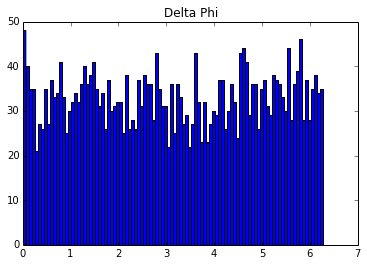
\includegraphics[width=\textwidth]{images/deltaphi}
        \subcaption{}
        \label{subfig:robust-deltaphi}
    \end{subfigure}
    \;
    \begin{subfigure}{0.3\textwidth}
        \centering
        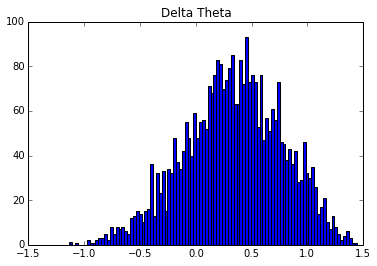
\includegraphics[width=\textwidth]{images/deltatheta}
        \subcaption{}
        \label{subfig:robust-deltatheta}
    \end{subfigure}
    \;
    \begin{subfigure}{0.3\textwidth}
        \centering
        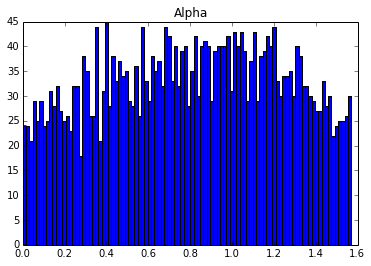
\includegraphics[width=\textwidth]{images/alpha}
        \subcaption{}
        \label{subfig:robust-alpha}
    \end{subfigure}
    \caption{Empirical results on the robustness of the proposed cosine of normals. (a) $\Delta \phi$ distribution (b) $\Delta \theta$ distribution (c) $\alpha$ distribution.}
    \label{fig:robust-properties}
\end{figure*}
%%%%%%%%%%%%%%%%%%%%%%%%%%%%%%%%%%%%%%%%%%%%%%%%%%%%%%%%
%%%%%%%%%%%%%%%%%%%%%%%%%%%%%%%%%%%%%%%%%%%%%%%%%%%%%%%%
\section{Properties of Normals}\label{sec:properties-of-normals}
%%%%%%%%%%%%%%%%%%%%%%%%%%%%%%%%%%%%%%%%%%%%%%%%%%%%%%%%
\begin{figure}[t]
    \centering
    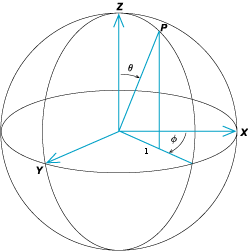
\includegraphics[width=0.6\columnwidth]{images/spherical-coordinates}
    \caption{The spherical coordinate system assumed in this paper.}
    \label{fig:spherical-coordinates}
\end{figure}
%%%%%%%%%%%%%%%%%%%%%%%%%%%%
It is important to clarify the properties of the subspace of normals, before attempting any statistical analysis on them. In particular, there are a number of ways in which we can parametrise normals at a given point. The simplest way to denote a normal is as a 3-component unit vector, $\boldsymbol{n} = [x, y, z]^T$. However, as is commonly noted in SFS literature, normals are uniquely defined by just two parameters. In SFS literature, these parameters are $p$ and $q$ and are related to the normal by the following relationship:
%%%%%%%%%%%%%%%%%%%%%%%%%%%%
\begin{equation}\label{eq:pq-representation}
    \boldsymbol{n} = \frac{[p, q, -1]^T}{\sqrt{p^2 + q^2 + (-1)^2}}
\end{equation}
%%%%%%%%%%%%%%%%%%%%%%%%%%%%
Here, $p$ and $q$ represent the local surface gradients $\left( \frac{\partial z}{\partial x}, \frac{\partial z}{\partial y} \right)$. However, as noted by Smith and Hancock in \cite{RefWorks:90}, a more useful depiction of normals is as points that lie on the surface of a unit sphere. Since each normal lies on this surface, we can uniquely define a given normal in terms of it's spherical coordinates, azimuth ($\phi$) and elevation ($\theta$), which is illustrated in Figure~\ref{fig:spherical-coordinates}. The azimuth angle represents rotation within the $xy$-plane and has range $[0, 2 \pi)$. The elevation angle represents inclination away from the $xy$-plane and has range $[-\frac{\pi}{2}, \frac{\pi}{2}]$. Conversion between a normal and the spherical coordinate system is given as follows
%%%%%%%%%%%%%%%%%%%%%%%%%%%%
\begin{equation}\label{eq:normal-to-spherical}
    \phi = \arctan{\frac{y}{x}}, \;\;\;\; \theta = \arccos{z}, \;\;\;\; r = 1
\end{equation}
%%%%%%%%%%%%%%%%%%%%%%%%%%%%
and from the spherical coordinates back to vector form is
%%%%%%%%%%%%%%%%%%%%%%%%%%%%
\begin{equation}\label{eq:spherical-to-normal}
    x = \sin{\theta} \cos{\phi}, \;\;\;\; y = \sin{\theta} \sin{\phi}, \;\;\;\; z = \cos{\theta}
\end{equation}
%%%%%%%%%%%%%%%%%%%%%%%%%%%%%%%%%%%%%%%%%%%%%%%%%%%%%%%%
\subsection{Cosine of Normals}\label{subsec:cosine-normals}
Our motivation for formulating normals in terms of angles is to enable the definition of a cosine based cost function. Tzimiropoulos et al. \cite{RefWorks:5} have shown that the sum of the cosines of gradient orientation differences (IGOs) represent a robust subspace. This is because, under the cosine kernel, the contribution of visually dissimilar areas sums to approximately zero. Therefore, since normals represent the orientation of a point on a surface, we seek to verify that visually dissimilar areas of normals will also sum to approximately zero. More formally
%%%%%%%%%%%%%%%%%%%%%%%%%%%%%%%%%%%%%%%%%%%%%%%%%%%%%%%%
\begin{equation}\label{eq:sum-of-cosines}
    \sum_{k \in P} \cos [\alpha (k)] \simeq 0
\end{equation}
%%%%%%%%%%%%%%%%%%%%%%%%%%%%
where $P$ is a set of visually dissimilar pixels and $k$ is an index in to $P$. Equation~\ref{eq:sum-of-cosines} will hold true in the case where the distribution of $\alpha (k)$ approximates a uniform distribution for a given range. However, we first need to identify the correct way to formulate $\alpha$. In fact, there are two ways to calculate the angular difference between normals.

In the following Sections~\ref{subsubsec:inner-product-normals} and \ref{subsubsec:spherical-normals} we assume that we are comparing two needle-maps, $\_1$ and $I_2$. Given that $I_1$ and $I_2$ are of the same size, we can then vectorise them and define an index $k$ to access each individual normal, $\boldsymbol{n}$. Finally, we assume we have identified a set of corresponding indexes, $P$, of visually dissimilar normals. Given $P$, we wish to define robust measures of the total similarity of $k \in P$.
%%%%%%%%%%%%%%%%%%%%%%%%%%%%%%%%%%%%%%%%%%%%%%%%%%%%%%%%
\subsubsection{Inner Product}\label{subsubsec:inner-product-normals}
A Hilbert space, $\hilbert$, is a generalisation of the Euclidean space to a potentially infinite dimensional vector space where an inner product is defined. Therefore, within any Hilbert space it is possible to measure the angle between two vectors in that space. In the case of normals, this inner product is defined as the standard three dimensional inner product
%%%%%%%%%%%%%%%%%%%%%%%%%%%%%%%%%%%%%%%%%%%%%%%%%%%%%%%%
\begin{equation}\label{eq:3d-inner-product}
    \cos \alpha = \frac{\boldsymbol{n}_1 \cdot \boldsymbol{n}_2}{\norm{\boldsymbol{n}_1} \norm{\boldsymbol{n}_2}}
\end{equation}
%%%%%%%%%%%%%%%%%%%%%%%%%%%%
where $\norm{\boldsymbol{n}_1} = \norm{\boldsymbol{n}_2} = 1$. Given Equation~\ref{eq:3d-inner-product} we can define our first robust measure of normals
%%%%%%%%%%%%%%%%%%%%%%%%%%%%
\begin{equation}\label{eq:cosine-inner-product}
    \sum_{k \in P} \cos[\alpha(k)]
\end{equation}
%%%%%%%%%%%%%%%%%%%%%%%%%%%%
Equation~\ref{eq:cosine-inner-product} will only be robust if the sum over $k$ is approximately zero. Given that $k$ is an index in to the set of visually dissimilar pixels, $P$, it is reasonable to assume that $\alpha$ will take any value within the range $[0, \frac{\pi}{2}]$ with equal probability. This is true if $\alpha$ is a realisation of a uniform distribution, $U(0, \frac{\pi}{2})$. In Figure~\ref{subfig:robust-alpha} we can see an example that suggests that $\alpha$ does appear to a approximate a uniform distribution.
%%%%%%%%%%%%%%%%%%%%%%%%%%%%%%%%%%%%%%%%%%%%%%%%%%%%%%%%
\subsubsection{Spherical difference}\label{subsubsec:spherical-normals}
As noted in Section~\ref{sec:properties-of-normals}, it is possible to uniquely define a normal given just two parameters. Due to the unit nature of normals, these two parameters are the azimuth, $\phi$, and elevation, $\theta$, angles as defined in Equation~\ref{eq:normal-to-spherical}. Since there are two angles to compare, we define our second robust measure as
%%%%%%%%%%%%%%%%%%%%%%%%%%%%%%%%%%%%%%%%%%%%%%%%%%%%%%%%
\begin{equation}\label{eq:cosine-spherical}
    \sum_{k \in P} \cos[\Delta \phi (k)] + \sum_{k \in P} \cos[\Delta \theta (k)]
\end{equation}
%%%%%%%%%%%%%%%%%%%%%%%%%%%%
where $\Delta \phi (k) = \phi_1 (k) - \phi_2 (k)$ and $\Delta \theta (k) = \theta_1 (k) - \theta_2 (k)$. In order for (\ref{eq:cosine-spherical}) to be robust, it would need to have properties similar to (\ref{eq:sum-of-cosines}). More formally, $\Delta \phi$ and $\Delta \theta$ would need to be realisations of uniform distributions of the form $U(0, 2 \pi)$ and $U(-\frac{\pi}{2}, \frac{\pi}{2})$. However, whilst this is true for the distribution of $\Delta \phi$ it is not true for the distribution of $\Delta \theta$, as shown in Figure~\ref{subfig:robust-deltatheta}. This is because $theta$ is not able to take any value in the range $[-\frac{\pi}{2}, \frac{\pi}{2}]$ for depth data, as the normals are assumed to be aligned pointing towards the camera plane. This means that, under normal circumstances, normals will not point away from the camera, thus limiting the range of valid $\Delta \theta$ values. However, the robustness of the $\Delta \phi$ outweighs the non-robust $\Delta \theta$ term, which we show extensively in the results section.

Since Equation~\ref{eq:cosine-spherical} involves the summation of two quantities, it does not represent a single measure that we might optimise within a LK framework. However, by observing that $\cos^2 \alpha + \sin^2 \alpha = 1 \; \forall \alpha$, then maximisation of (\ref{eq:cosine-spherical}) is equivalent to the minimisation of
%%%%%%%%%%%%%%%%%%%%%%%%%%%%
\begin{equation}\label{eq:minimise-spherical}
       \sum_{k \in P} \Big[ 
        \begin{pmatrix}
            \cos \phi_1 (k) \\ 
            \sin \phi_1 (k) \\
            \cos \theta_1 (k) \\ 
            \sin \theta_1 (k)
        \end{pmatrix}
        -
        \begin{pmatrix}
            \cos \phi_2 (k) \\ 
            \sin \phi_2 (k) \\
            \cos \theta_2 (k) \\ 
            \sin \theta_2 (k)
        \end{pmatrix}
        \Big] ^2
\end{equation}
%%%%%%%%%%%%%%%%%%%%%%%%%%%%
where
%%%%%%%%%%%%%%%%%%%%%%%%%%%%
\begin{equation}
    \begin{aligned}\label{eq:normalised-spherical}
        \cos \phi_i   &=& \tilde{x}_i \;\;\;\; \sin \phi_i   &=& \tilde{y}_i \\
        \cos \theta_i &=& \tilde{z}_i \;\;\;\; \sin \theta_i &=& \sqrt{1 - {\tilde{z}_i}^2}
    \end{aligned}
\end{equation}
%%%%%%%%%%%%%%%%%%%%%%%%%%%%
and $\tilde{x}_i = \frac{x_i}{\sqrt{x_i^2 + y_i^2}}$, $\tilde{y}_i = \frac{y_i}{\sqrt{x_i^2 + y_i^2}}$, $\tilde{z}_i = \frac{z_i}{\sqrt{x_i^2 + y_i^2 + z_i^2}}$. This normalisation of each component is done to suppress any magnitude contribution from orientation.
%%%%%%%%%%%%%%%%%%%%%%%%%%%%%%%%%%%%%%%%%%%%%%%%%%%%%%%%
%%%%%%%%%%%%%%%%%%%%%%%%%%%%%%%%%%%%%%%%%%%%%%%%%%%%%%%%
\begin{figure}[t]
    \centering
    \begin{subfigure}{0.45\columnwidth}
        \centering
        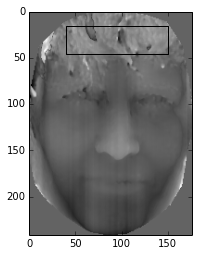
\includegraphics[width=\columnwidth]{images/face1}
        \subcaption{}
        \label{subfig:robust-face1}
    \end{subfigure}
    \hfill
    \begin{subfigure}{0.45\columnwidth}
        \centering
        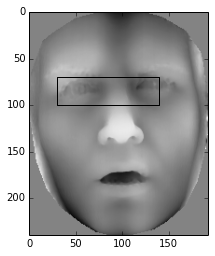
\includegraphics[width=\columnwidth]{images/face2}
        \subcaption{}
        \label{subfig:robust-face2}
    \end{subfigure}
    \caption{The images used to produce the results in Figure~\ref{fig:robust-properties}.}
    \label{fig:robust-faces}
\end{figure}
%%%%%%%%%%%%%%%%%%%%%%%%%%%%%%%%%%%%%%%%%%%%%%%%%%%%%%%%
%%%%%%%%%%%%%%%%%%%%%%%%%%%%%
%%%%%%%%%%%%%%%%%%%%%%%%%%%%%%%%%%%%%%%%%%%%%%%%%%%%%%%%%%%%%%
\section{Proof of concept: Robust LK cost functions}\label{sec:proof-of-concept-lk}
%%%%%%%%%%%%%%%%%%%%%%%%%%%%%%%%%%%%%%%%%%%%%%%%%%%%%%%%%%%%%%
The original forward additive $\ltwo$ LK algorithm \cite{RefWorks:71,RefWorks:10} seeks to minimise the SSD between a given template image and an input image by minimising the sum of the squared pixel differences:
%%%%%%%%%%%%%%%%%%%%%%%%%%%%%%%
\begin{equation}\label{eq:l2-lk-fa}
    \argmin_{\p} \norm{I(\p) - T(\zero)}^2
\end{equation}
%%%%%%%%%%%%%%%%%%%%%%%%%%%%%%%
where $T(\zero)$ is the unwarped reference template image. Due to the non-linear nature of (\ref{eq:l2-lk-fa}) with respect to $\p$, (\ref{eq:l2-lk-fa}) is linearised by taking the first order Taylor series expansion. By iteratively solving for some small $\Delta \p$ update to $\p$, the objective function becomes
%%%%%%%%%%%%%%%%%%%%%%%%%%%%%%%
\begin{equation}\label{eq:l2-lk-linearised-fa}
    \argmin_{\p} \norm{I(\p) + \nabla I \frac{\partial \mathcal{W}}{\partial \p} \Delta \p - T(\zero)}^2
\end{equation}
%%%%%%%%%%%%%%%%%%%%%%%%%%%%%%%
where $\nabla I$ is the gradient over each dimension of $I(\zero)$ warped into the frame of $T$ by the current warp estimate $\mathcal{W}(\boldsymbol{x};\p)$.  $\frac{\partial \mathcal{W}}{\partial \p}$ is the Jacobian of the warp and represents the first order partial derivatives of the warp with respect to each parameter. $\nabla I \frac{\partial \mathcal{W}}{\partial \p}$ is commonly referred to as the steepest descent images. We will express the steepest descent images as $\frac{\partial I(\p)}{\partial \p}$. Equation~\ref{eq:l2-lk-linearised-fa} is now solvable by assuming the gauss-newton approximation to the Hessian, $\boldsymbol{H} = \left[ {\frac{\partial I(\p)}{\partial \p}}^T \frac{\partial I(\p)}{\partial \p} \right]$:
%%%%%%%%%%%%%%%%%%%%%%%%%%%%%%%
\begin{equation}\label{eq:l2-lk-gauss-newton-fa}
    \Delta \p = \boldsymbol{H}^{-1} \frac{\partial I(\p)}{\partial \p}^T \left[ T(\zero) - I(\p) \right]
\end{equation}
%%%%%%%%%%%%%%%%%%%%%%%%%%%%%%%
Equation~\ref{eq:l2-lk-gauss-newton-fa} can then be solved by iteratively updating $\p \leftarrow \p + \Delta \p$ until convergence.
%%%%%%%%%%%%%%%%%%%%%%%%%%%%%%%%%%%%%%%%%%%%%%%%%%%%%%%%%%%%%%
\subsection{ECC LK Fitting}\label{subsec:lk-ecc}
%%%%%%%%%%%%%%%%%%%%%%%%%%%%%%%%%%%%%%%%%%%%%%%%%%%%%%%%%%%%%%
The ECC measure, proposed by Evangelidis and Psarakis \cite{RefWorks:59}, seeks to be invariant to illumination variations within the input and template image. This is done by suppressing the magnitude of each pixel through normalisation. In \cite{RefWorks:59}, they proved that maximisation of
%%%%%%%%%%%%%%%%%%%%%%%%%%%%%%%
\begin{equation}\label{eq:ecc-lk-max}
   \argmax_{\p} \frac{I(\p)^T T(\zero)}{\norm{I(\p)} \norm{T(\zero)}}
\end{equation}
%%%%%%%%%%%%%%%%%%%%%%%%%%%%%%%
is equivalent to minimisation of
%%%%%%%%%%%%%%%%%%%%%%%%%%%%%%%
\begin{equation}\label{eq:ecc-lk-min}
    \argmin_{\p} \left \lVert \frac{I(\p)}{\norm{I(\p)}} - \frac{T(\zero)}{\norm{T(\zero)}} \right \rVert^2
\end{equation}
%%%%%%%%%%%%%%%%%%%%%%%%%%%%%%%
Assuming a delta update as before and linearising in a similar manner to (\ref{eq:l2-lk-linearised-fa}) results in
%%%%%%%%%%%%%%%%%%%%%%%%%%%%%%%
\begin{equation}\label{eq:ecc-lk-linearised}
    \argmin_{\p} \hat{T} \frac{I(\p) + \frac{\partial I(\p)}{\partial \p} \Delta \p}{\norm{{I(\p) + \frac{\partial I(\p)}{\partial \p} \Delta \p}}}
\end{equation}
%%%%%%%%%%%%%%%%%%%%%%%%%%%%%%%
where $\hat{T} = \frac{T(\zero)}{\norm{T(\zero)}}$.
Evangelidis and Psarakis \cite{RefWorks:59} give a very comprehensive proof of the upper bound of Equation~\ref{eq:ecc-lk-linearised}, which yields the following solution for $\Delta \p$
%%%%%%%%%%%%%%%%%%%%%%%%%%%%%%%
%%%%%%%%%%%%%%%%%%%%%%%%%%%%%%%
\begin{equation}\label{eq:ecc-lk-gauss-newton-fa}
    \Delta \p = \boldsymbol{H}^{-1} \frac{\partial I(\p)}{\partial \p}^{\top} \left[ \frac{\norm{I(\p)}^2 - I(\p)^{\top} \boldsymbol{Q} I(\p)}{\hat{T}^{\top} I(\p) - \hat{T}^{\top} \boldsymbol{Q} I(\p)} \hat{T} - I(\p) \right]
\end{equation}
%%%%%%%%%%%%%%%%%%%%%%%%%%%%%%%
where $Q$ is an orthogonal projection operator on the Jacobian, $\J = \frac{\partial I(\p)}{\partial \p}$, defined as $\boldsymbol{Q} = \J (\J^\top \J)^{-1} \J^\top$.

In fact, the $\Delta p$ update given in \cite{RefWorks:59} is more complex than (\ref{eq:ecc-lk-gauss-newton-fa}), as it seeks to find an upper bound on the correlation between the two images. However, in the case where (\ref{eq:ecc-lk-gauss-newton-fa}) does not apply, it is unlikely that the algorithm is unable to recover and so we choose to concentrate on the provided solution.
%%%%%%%%%%%%%%%%%%%%%%%%%%%%%%%%%%%%%%%%%%%%%%%%%%%%%%%%%%%%%%
\subsection{Inverse Compositional LK}\label{subsec:lk-ic}
%%%%%%%%%%%%%%%%%%%%%%%%%%%%%%%%%%%%%%%%%%%%%%%%%%%%%%%%%%%%%%
The inverse compositional algorithm, proposed by Baker and Matthews \cite{RefWorks:74}, performs a compositional update of the warp and linearises over the template rather than the input image. Linearisation of the template image causes the gradient in the steepest descent images term to become fixed. The compositional update of the warp assumes linearisation of the term $\frac{\partial \mathcal{W}(\boldsymbol{x};\zero)}{\partial \p}$, which is also fixed. Therefore, the entire Jacobian term, and by extension the Hessian matrix, are also fixed. Similar to the $\ltwo$ SSD algorithm described above
%%%%%%%%%%%%%%%%%%%%%%%%%%%%%%%
\begin{equation}\label{eq:l2-lk-ic}
    \argmin_{\p} \norm{T(\Delta \p) - I(\p)}^2
\end{equation}
%%%%%%%%%%%%%%%%%%%%%%%%%%%%%%%
where we notice that the roles of the template and input image have been swapped. Assuming an inverse compositional update to the warp, $\mathcal{W}(\boldsymbol{x};\p) \leftarrow \mathcal{W}(\boldsymbol{x};\p) \circ \mathcal{W}(\boldsymbol{x};\Delta \p)^{-1}$ and linearisaton around the template
%%%%%%%%%%%%%%%%%%%%%%%%%%%%%%%
\begin{equation}\label{eq:l2-lk-linearised-ic}
    \argmin_{\p} \norm{I(\p) - \frac{\partial T(\zero)}{\partial \p} \Delta \p - T(\zero)}^2
\end{equation}
%%%%%%%%%%%%%%%%%%%%%%%%%%%%%%%
Solving for $\Delta \p$ is identical to (\ref{eq:l2-lk-gauss-newton-fa}), except the Jacobian and Hessian have been pre-computed
%%%%%%%%%%%%%%%%%%%%%%%%%%%%%%%
\begin{equation}\label{eq:l2-lk-gauss-newton-ic}
    \Delta \p = \boldsymbol{H}^{-1} \frac{\partial T(\zero)}{\partial \p}^T \left[ I(\p) - T(\zero) \right]
\end{equation}
%%%%%%%%%%%%%%%%%%%%%%%%%%%%%%%
The ECC can also be described as an inverse compositional algorithm, by performing the same update to the warp and simply swapping the roles of the template and reference image. In short, solving ECC in the inverse compositional case becomes
%%%%%%%%%%%%%%%%%%%%%%%%%%%%%%%
\begin{equation}\label{eq:ecc-lk-gauss-newton-ic}
    \Delta \p = \boldsymbol{H}^{-1} \frac{\partial T(\zero)}{\partial \p}^{\top} \left[ \frac{\norm{\hat{T}}^2 - \hat{T}^{\top} \boldsymbol{Q} \hat{T}}{I(\p)^{\top} \hat{T} - I(\p)^{\top} \boldsymbol{Q} \hat{T}} I(\p) - \hat{T} \right]
\end{equation}
%%%%%%%%%%%%%%%%%%%%%%%%%%%%%%%
where $\boldsymbol{Q}$ is as before, except $\J = \frac{\partial T(\zero)}{\partial \p}$. Any term involving $\hat{T}$ is fixed and pre-computable, so the reduction of calculations per-iteration is substantial.

It is worth noting that not every family of warps is suitable for the inverse compositional approach. The warp must belong to a family that forms a group, and the identity warp must exist in the set of possible warps. For more complex warps, such as piecewise affine and thin plate spline warping, approximations to the inverse compositional updates have been proposed \cite{RefWorks:227, RefWorks:277}.
%%%%%%%%%%%%%%%%%%%%%%%%%%%%%%%%%%%%%%%%%%%%%%%%%%%%%%%%%%%%%%
\subsection{Inner Product ECC LK}\label{subsec:lk-inner-product}
%%%%%%%%%%%%%%%%%%%%%%%%%%%%%%%%%%%%%%%%%%%%%%%%%%%%%%%%%%%%%%
Combining the inner product relationship between normals, as described in Equation~\ref{eq:cosine-inner-product} with the ECC objective function yields a robust objective function for depth maps. By defining $G_I$ and $G_T$ as the normals computed from the input and template depth maps respectively, we can define the following forwards additive objective function
%%%%%%%%%%%%%%%%%%%%%%%%%%%%%%%
\begin{equation}\label{eq:ip-ecc-lk-max}
   \argmax_{\p} \frac{G_I(\zero)^{\top} G_T(\p)}{\norm{G_I(\zero)} \norm{G_T(\p)}}
\end{equation}
%%%%%%%%%%%%%%%%%%%%%%%%%%%%%%%
and following the same logic as in (\ref{eq:ecc-lk-min}), we can minimise (\ref{eq:ip-ecc-lk-max}) as
%%%%%%%%%%%%%%%%%%%%%%%%%%%%%%%
\begin{equation}\label{eq:ip-ecc-lk-min}
   \argmin_{\p} \left \lVert \frac{G_I(\p)}{\norm{G_I(\p)}} - \frac{G_T(\zero)}{\norm{G_T(\zero)}} \right \rVert^2
\end{equation}
%%%%%%%%%%%%%%%%%%%%%%%%%%%%%%%
However, $G_I(\p)$ and $G_T(\zero)$ are formed of the concatenated components of all the normals within the needle-maps. Therefore, when linearising $G_I$, care must be taken to treat each component separately. Since $G_I$ is composed of multiple components, there will be extra derivatives to calculate via the chain rule. Formally, linearising (\ref{eq:ip-ecc-lk-min}) with respect to $G_I$ yields
%%%%%%%%%%%%%%%%%%%%%%%%%%%%%%%
\begin{equation}\label{eq:ip-ecc-lk-linearised}
    \argmin_{\p} \hat{G_T} \frac{G_I(\p) + \boldsymbol{J}_G \Delta \p}{\norm{{G_I(\p) + \boldsymbol{J}_G \Delta \p}}}
\end{equation}
%%%%%%%%%%%%%%%%%%%%%%%%%%%%%%%
where $\boldsymbol{J}_G$ is the matrix formed by correctly computing the derivative of $G_I$ with respect to each component of $G_I$. For example, given that $G_{I,x}(\p)$ is a vector formed of the $x$-components of the normals in the input needle-map and $\hat{G}_{I,x}(\p) = \frac{G_{I,x}(\p)}{\norm{G_I(\p)}}$, the true derivative of $\hat{G}_{I,x}(\p)$ is
%%%%%%%%%%%%%%%%%%%%%%%%%%%%%%%
\begin{equation}\label{eq:ip-ecc-chain-rule}
    \begin{aligned}
        \frac{\partial \hat{G}_{I,x}(\p)}{\partial \p}          &= \frac{\partial \hat{G}_{I,x}(\p)}{\partial G_{I,x}(\p)} \frac{\partial G_{I,x}(\p)}{\partial \p} \\
        \frac{\partial \hat{G}_{I,x}(\p)}{\partial G_{I,x}(\p)} &= \frac{G_{I,y}(\p)^2 + G_{I,z}(\p)^2}{\left(G_{I,x}(\p)^2 + G_{I,y}(\p)^2 + G_{I,z}(\p)^2 \right)^{\sfrac{3}{2}}}
    \end{aligned}
\end{equation}
%%%%%%%%%%%%%%%%%%%%%%%%%%%%%%%
where $\frac{\partial G_{I,x}(\p)}{\partial \p}$ is equivalent to $\frac{\partial I(\p)}{\partial \p}$ in the depth domain. However, $\nabla G_{I,x}$ inside $\frac{\partial G_{I,x}(\p)}{\partial \p} = \nabla G_{I,x} \frac{\partial \mathcal{W}}{\partial \p}$ represents the gradient over only the $x$-component of the needle-map, and is equivalent to the second order derivative of the depth map with respect to $x$. 

Since $\frac{\partial G_{I,x}(\p)}{\partial \p}$ is a matrix and $\frac{\partial \hat{G}_{I,x}(\p)}{\partial G_{I,x}(\p)}$ is a vector, we multiply the two using a hadamard product. However, $\frac{\partial \hat{G}_{I,x}(\p)}{\partial G_{I,x}(\p)}$ must first form a matrix, $\boldsymbol{J}_x$, of size $D \times p$ by repeating the vector $p$ to form the columns. Finally the total $x$-component Jacobian is given by $\boldsymbol{J}_{G,x} = \boldsymbol{J}_x \odot \frac{\partial G_{I,x}(\p)}{\partial \p}$.

Given that $\boldsymbol{J}_{G,i} \forall i \in \left\{ x,y,z \right\}$ have been calculated, the total derivative term is given by $\boldsymbol{J}_G = \left[ \boldsymbol{J}_{G,x}, \boldsymbol{J}_{G,y}, \boldsymbol{J}_{G,z} \right]^T$. Solving for $\Delta \p$ is now identical to the ECC formulation:
%%%%%%%%%%%%%%%%%%%%%%%%%%%%%%%
\begin{equation}\label{eq:ip-ecc-lk-gauss-newton-ic}
    \Delta \p = \boldsymbol{H}^{-1} \boldsymbol{J}_G^{\top} \left[ \frac{\norm{\hat{G_T}}^2 - \hat{G_T}^{\top} \boldsymbol{Q} \hat{G_T}}{G_I(\p)^{\top} \hat{G_T} - G_I(\p)^{\top} \boldsymbol{Q} \hat{G_T}} G_I(\p) - \hat{G_T} \right]
\end{equation}
%%%%%%%%%%%%%%%%%%%%%%%%%%%%%%%
where $\hat{G_T} = \frac{G_T}{\norm{G_T}}$. Since the update step is identical to the one given in (\ref{eq:ecc-lk-gauss-newton-ic}) it is trivial to reformulate the inner product ECC in an inverse compositional form by following a derivation identical to Section~\ref{subsec:lk-ic}.
%%%%%%%%%%%%%%%%%%%%%%%%%%%%%%%%%%%%%%%%%%%%%%%%%%%%%%%%%%%%%%
\subsection{Spherical SSD LK}\label{subsec:lk-spherical}
%%%%%%%%%%%%%%%%%%%%%%%%%%%%%%%%%%%%%%%%%%%%%%%%%%%%%%%%%%%%%%
In contrast to the inner product derivation in the previous section, the spherical representation of normals requires the optimisation of two separate cosine correlations. In theory, it would be possible to solve for each cosine separately in the same way the inner product objective function is defined. However, in the interest of solving a single objective function, we use the relationship defined by Equation~\ref{eq:minimise-spherical}. For notational simplicity, let $\tilde{sz} = \sqrt{1 - \tilde{z}^2}$. Therefore, we define our forward additive objective function as
%%%%%%%%%%%%%%%%%%%%%%%%%%%%
\begin{equation}\label{eq:spher-ssd}
    \argmin_{\p} \norm{\tilde{G}_I(\p) - \tilde{G}_T(\zero)}^2
\end{equation}
%%%%%%%%%%%%%%%%%%%%%%%%%%%%
where $\tilde{G}_I(\p) = \left[  \tilde{x}_I(\p), \tilde{y}_I(\p), \tilde{z}_I(\p), \tilde{sz}_I(\p) \right]^T$ and $\tilde{G}_T(\zero) = \left[ \tilde{x}_T(\zero), \tilde{y}_T(\zero), \tilde{z}_T(\zero), \tilde{sz}_T(\zero) \right]^T$, the concatenated vectors of each normalised component.

Similar to the derivation in Section~\ref{subsec:lk-inner-product}, the Jacobian must be taken over each component and thus linearising around $\tilde{G}_I(\p)$ yields
%%%%%%%%%%%%%%%%%%%%%%%%%%%%%%%
\begin{equation}\label{eq:spher-ssd-linearised}
    \argmin_{\p} \norm{\tilde{G}_I(\p) + \tilde{\boldsymbol{J}}_G \Delta \p - \tilde{G}_T(\zero)}^2
\end{equation}
%%%%%%%%%%%%%%%%%%%%%%%%%%%%%%%
where $\tilde{\boldsymbol{J}}_G = \left[ \tilde{\boldsymbol{J}}_{G,x}, \tilde{\boldsymbol{J}}_{G,y}, \tilde{\boldsymbol{J}}_{G,z}, \tilde{\boldsymbol{J}}_{G,sz} \right]^T$. Unlike in Section~\ref{subsec:lk-inner-product}, the calculation of each Jacobian is not identical due to the different normalisation procedure taken for each component. Given that $\boldsymbol{J}_{G,x} = \boldsymbol{J}_x \odot \frac{\partial G_{I,x}(\p)}{\partial \p}$ and $\boldsymbol{J}_x$ is as described previously, we give the derivation of each $\boldsymbol{J}_i \forall i \in \left\{ x,y,z,sz \right\}$ as:
%%%%%%%%%%%%%%%%%%%%%%%%%%%%%%%
\begin{equation}\label{eq:spher-ssd-chain-rule}
    \begin{aligned}
        \boldsymbol{J}_x    &= \frac{G_{I,y}(\p)^2}{\left(G_{I,x}(\p)^2 + G_{I,y}(\p)^2 + G_{I,z}(\p)^2 \right)^{\sfrac{3}{2}}} \\
        \boldsymbol{J}_y    &= \frac{G_{I,x}(\p)^2}{\left(G_{I,x}(\p)^2 + G_{I,y}(\p)^2 + G_{I,z}(\p)^2 \right)^{\sfrac{3}{2}}} \\
        \boldsymbol{J}_z    &= \frac{G_{I,x}(\p)^2 + G_{I,y}(\p)^2}{\left(G_{I,x}(\p)^2 + G_{I,y}(\p)^2 + G_{I,z}(\p)^2 \right)^{\sfrac{3}{2}}} \\
        \boldsymbol{J}_{sz} &= - \frac{G_{I,z}(\p) \left( \frac{G_{I,x}(\p)^2 + G_{I,y}(\p)^2}{G_{I,x}(\p)^2 + G_{I,y}(\p)^2 + G_{I,z}(\p)^2} \right)^{\sfrac{3}{2}}}{G_{I,x}(\p)^2 + G_{I,y}(\p)^2}
    \end{aligned}
\end{equation}
%%%%%%%%%%%%%%%%%%%%%%%%%%%%%%%
Now, given the definitons of the correct Jacobians per component, we can solve (\ref{eq:spher-ssd-linearised}) as:
%%%%%%%%%%%%%%%%%%%%%%%%%%%%%%%
\begin{equation}\label{eq:spher-ssd-gauss-newton}
    \Delta \p = \boldsymbol{H}^{-1} \tilde{\boldsymbol{J}}_G^T \left[ \tilde{G}_T(\zero) - \tilde{G}_I(\p) \right]
\end{equation}
%%%%%%%%%%%%%%%%%%%%%%%%%%%%%%%
Given that the update in (\ref{eq:spher-ssd-gauss-newton}) is identical to that of (\ref{eq:l2-lk-gauss-newton-fa}), it would be trivial to formulate an inverse compositional form of this residual by following the steps described in Section~\ref{subsec:lk-ic}.
%%%%%%%%%%%%%%%%%%%%%%%%%%%%%
\section{A Kernel-PCA framework for normals}\label{sec:kernel-pca-for-normals}
Computing principal components on a subspace of normals is non-trivial due to the fact that normals exist as points lying on the surface of a 2-sphere. For this reason, it is claimed that linear statistical analysis techniques such as PCA cannot be performed directly on normals \footnote{In particular because the definition of a mean is not well defined in arbitrary dimensional spheres}. In order to alleviate this problem, mapping techniques from the unit sphere to an approximate Euclidean space have been proposed \cite{RefWorks:86,RefWorks:90,RefWorks:100}. The most popular proposed techniques are the Azimuthal Equidistant Projection (AEP) and Principal Geodesic Analysis (PGA).  However, in KPCA, we only need to define a kernel that provides an inner product between two vectors in a space. Following the properties of normals described in Section~\ref{sec:properties-of-normals}, we derive kernels for the existing AEP and PGA techniques and show the connection between the angular difference between normals and robust kernels.

We maintain the notation outlined in Section~\ref{subsec:notation-normals} when defining our kernels. Once a vector, $\boldsymbol{x}_k$, has been mapped in to the feature space, we refer to the concatenated feature vectors as $\boldsymbol{v}_k$. The vector $\boldsymbol{v}_k$ will have as many components as the feature space requires.
%%%%%%%%%%%%%%%%%%%%%%%%%%
\subsection{Kernel PCA}\label{sec:kpca}
Given a set of, $K$, $F$-dimensional data vectors stacked in a matrix $ \boldsymbol{X} = [\boldsymbol{x}_1, \ldots, \boldsymbol{x}_K] \in \R^F$, we assume the existence of a positive semi-definite kernel function $k(\circ, \circ) : \R^F \times \R^F \rightarrow \R$. Given that $k(\circ, \circ)$ is positive semi-definite we can use it to define the inner product in an arbitrary dimensional Hilbert space, $\hilbert$, which we will call the feature space. There then exists an implicit mapping, $\Phi$, from the input space $\R^F$ to the feature space, $\hilbert$:
%%%%%%%%%%%%%%%%%%%%%%%%%%%%%%%%%%%%%%%%%%%%
\begin{equation}
    \begin{aligned}\label{eq:implicit-map}
        \Phi : \R^F \rightarrow \hilbert, \; \; \boldsymbol{x} \rightarrow \Phi(\boldsymbol{x})
    \end{aligned}
\end{equation}
%%%%%%%%%%%%%%%%%%%%%%%%%%%%%%%%%%%%%%%%%%%%
Due to the often implicit nature of the mapping $\Phi$, we need only the kernel function since $\langle \Phi(\boldsymbol{x}_i), \Phi(\boldsymbol{x}_j) \rangle  = k (\boldsymbol{x}_i, \boldsymbol{x}_j)$, the so-called kernel trick. Now, component analysis within the feature space is equivalent to
%%%%%%%%%%%%%%%%%%%%%%%%%%%%%%%%%%%%%%%%%%%%
\begin{equation}
    \begin{aligned}\label{eq:feature-space-pca}
        \underset{\boldsymbol{U}_\Phi}{\arg\max} \; \boldsymbol{U}_\Phi^T \bar{\boldsymbol{X}}_\Phi \bar{\boldsymbol{X}}_\Phi^T \boldsymbol{U}_\Phi \qquad \text{s.t.} \; \boldsymbol{U}_\Phi^T \boldsymbol{U}_\Phi = \boldsymbol{I}
    \end{aligned}
\end{equation}
%%%%%%%%%%%%%%%%%%%%%%%%%%%%%%%%%%%%%%%%%%%%
where $\boldsymbol{U}_\Phi = [\boldsymbol{U}_\Phi^1, ..., \boldsymbol{U}_\Phi^P] \in \hilbert$, $\boldsymbol{m}_\Phi = \frac{1}{K} \sum \limits_{i=1}^K \Phi(\boldsymbol{x_i})$ and $\bar{\boldsymbol{X}}_\Phi = [\Phi(\boldsymbol{x_i}) - \boldsymbol{m}_\Phi, ..., \Phi(\boldsymbol{x_K}) - \boldsymbol{m}_\Phi]$.

By noting that $\boldsymbol{\bar{X}}_\Phi \boldsymbol{\bar{X}}_\Phi^T = (\boldsymbol{X}_\Phi \boldsymbol{M}) (\boldsymbol{X}_\Phi \boldsymbol{M})^T$, where $\boldsymbol{M} = \boldsymbol{I} - \frac{1}{K} \boldsymbol{1} \boldsymbol{1}^T$ and $\boldsymbol{1}$ represents a vector of ones, we can find $\boldsymbol{U}_\Phi$ by performing eigenanalysis on $\bar{\boldsymbol{X}}_\Phi^T \bar{\boldsymbol{X}}_\Phi$. Therefore,
%%%%%%%%%%%%%%%%%%%%%%%%%%%%%%%%%%%%%%%%%%%%
\begin{equation}
    \begin{aligned}\label{eq:x-bar-corr}
        \boldsymbol{\bar{X}}_\Phi^T \boldsymbol{\bar{X}}_\Phi = \boldsymbol{V} \boldsymbol{\Lambda} \boldsymbol{V}^T \boldsymbol{U}_{\Phi} &= \boldsymbol{\bar{X}}_\Phi^T \boldsymbol{V} \boldsymbol{\Lambda}^{-\frac{1}{2}}
    \end{aligned}
\end{equation}
%%%%%%%%%%%%%%%%%%%%%%%%%%%%%%%%%%%%%%%%%%%%
Though $\boldsymbol{U}_\Phi$ can be defined, it cannot be calculated explicitly. However, we can compute the KPCA-transformed feature vector $\boldsymbol{\tilde{y}} = [\boldsymbol{y}_1, ..., \boldsymbol{y}_K]$ by:
%%%%%%%%%%%%%%%%%%%%%%%%%%%%%%%%%%%%%%%%%%%%
\begin{equation}
    \begin{aligned}\label{eq:projections}
        \boldsymbol{\tilde{y}} = \boldsymbol{U}_\Phi^T \Phi(\boldsymbol{y}) &= \boldsymbol{\Lambda}^{-\frac{1}{2}} \boldsymbol{V}^T \boldsymbol{\bar{X}}_\Phi^T \Phi(\boldsymbol{y}) \\
        &= \boldsymbol{\Lambda}^{-\frac{1}{2}} \boldsymbol{V}^T \boldsymbol{M} \boldsymbol{X}_\Phi^T \Phi(\boldsymbol{y})
    \end{aligned}
\end{equation}
%%%%%%%%%%%%%%%%%%%%%%%%%%%%%%%%%%%%%%%%%%%%
We can, therefore, define the projection in terms of the kernel function
%%%%%%%%%%%%%%%%%%%%%%%%%%%%%%%%%%%%%%%%%%%%
\begin{equation}\label{eq:kernel-vector}
        \boldsymbol{X}_\Phi^T \Phi(\boldsymbol{y}) = \left[ k(\boldsymbol{y}_1, \boldsymbol{x}_1), \ldots, k(\boldsymbol{y}_K, \boldsymbol{x}_K) \right]^T
\end{equation}
%%%%%%%%%%%%%%%%%%%%%%%%%%%%%%%%%%%%%%%%%%%%
Reconstruction of a vector can be performed by
%%%%%%%%%%%%%%%%%%%%%%%%%%%%%%%%%%%%%%%%%%%%
\begin{equation}\label{eq:vector-reconstruction}
        \boldsymbol{\tilde{X}} = {\Phi}^{-1} \left( \boldsymbol{U}_{\Phi} {\boldsymbol{U}_{\Phi}}^T (\Phi(\boldsymbol{x}) - \boldsymbol{m}_{\Phi}) + \boldsymbol{m}_{\Phi} \right)
\end{equation}
%%%%%%%%%%%%%%%%%%%%%%%%%%%%%%%%%%%%%%%%%%%%
Unfortunately, since ${\Phi}^{-1}$ rarely exists or is extremely expensive to compute, performing reconstruction using (\ref{eq:vector-reconstruction}) is not generally feasible. In these cases, reconstruction can be performed by means of pre-images \cite{RefWorks:254}. However, in the case of the kernels we propose for normals, ${\Phi}^{-1}$ does exist and explicit mapping between the space of normals and kernel space is performed. Finally, we should note here that in the general KPCA framework it is not necessary to subtract the mean. In this case, KPCA can be seen in the perspective of metric multi-dimensional scaling \cite{RefWorks:253}.
%%%%%%%%%%%%%%%%%%%%%%%%%%
%%%%%%%%%%%%%%%%%%%%%%%%%%%%%%%%%%%%%%%%%%%%%%%%%%%%%%%%%%%%%%%%%%%%%%%%%%%%%%%%%%%%%%%%
\subsection{Inner Product Kernel}\label{subsec:ip-kernel}
%%%%%%%%%%%%%%%%%%%%%%%%%%%%%%%%%%%%%%%%%%%%%%%%%%%%%%%%%%%%%%%%%%%%%%%%%%%%%%%%%%%%%%%%
Given that the Euclidean inner product is well defined for normals, as described in (\ref{eq:3d-inner-product}), we can define a kernel of the form
%%%%%%%%%%%%%%%%%%%%%%%%%%%%%%%%%%%%%%%%%%%%
\begin{equation}\label{eq:ip-cosine-kernel}
    k(\boldsymbol{x}_i, \boldsymbol{x}_j) = \sum^K_k {\boldsymbol{n}_k^i}^T \boldsymbol{n}_k^j = \sum^K_k \cos \alpha^{ij}_k
\end{equation}
%%%%%%%%%%%%%%%%%%%%%%%%%%%%%%%%%%%%%%%%%%%%
where $\alpha^{ij}_k = \langle \boldsymbol{n}^i_k, \boldsymbol{n}^j_k \rangle$.

Subtracting the mean would affect the calculation of the cosine and thus would not preserve the cosine distance. Therefore, we note that the inner product mapping is equivalent to performing PCA without subtracting the mean. We refer to this kernel as the inner product (IP) kernel, and denote it as:
%%%%%%%%%%%%%%%%%%%%%%%%%%%%%%%%%%%%%%%%%%%%
\begin{equation}\label{eq:ip-kernel}
    \ip = \boldsymbol{x}_k
\end{equation}
%%%%%%%%%%%%%%%%%%%%%%%%%%%%%%%%%%%%%%%%%%%%
We can explicitly define the inverse mapping for the inner product as the normalisation of each individual normal within the feature space vector, $\boldsymbol{v}_k$:
%%%%%%%%%%%%%%%%%%%%%%%%%%%%%%%%%%%%%%%%%%%%
\begin{equation}\label{eq:inv-ip-kernel}
    \invip = \left[ x_k^1, y_k^1, z_k^1, \ldots, x_k^N, y_k^N, z_k^N \right]^T
\end{equation}
%%%%%%%%%%%%%%%%%%%%%%%%%%%%%%%%%%%%%%%%%%%%

After computing $\ip$, we estimate $\boldsymbol{U}_{IP}$ from (\ref{eq:feature-space-pca}) and set $\boldsymbol{M} = \boldsymbol{I}$. Reconstruction of a test vector of normals $\boldsymbol{x}$ is performed via
%%%%%%%%%%%%%%%%%%%%%%%%%%%%%%%%%%%%%%%%%%%%
\begin{equation}\label{eq:ip-reconstruction}
   \tilde{\boldsymbol{x}} = {\Phi_{IP}}^{-1} \left( \boldsymbol{U}_{IP} {\boldsymbol{U}_{IP}}^T \Phi_{IP}(\boldsymbol{x}) \right)
\end{equation}
%%%%%%%%%%%%%%%%%%%%%%%%%%%%%%%%%%%%%%%%%%%%
%%%%%%%%%%%%%%%%%%%%%%%%%%%%%%%%%%%%%%%%%%%%%%%%%%%%%%%%%%%%%%%%%%%%%%%%%%%%%%%%%%%%%%%%
\subsection{AEP Kernel}\label{subsec:aep-kernel}
%%%%%%%%%%%%%%%%%%%%%%%%%%%%%%%%%%%%%%%%%%%%%%%%%%%%%%%%%%%%%%%%%%%%%%%%%%%%%%%%%%%%%%%%
The azimuthal equidistant projection (AEP) \cite{RefWorks:102,RefWorks:90} is a cartographic projection often used for creating charts centred on the north pole. The projection has the useful property that all lines that pass through the centre of the projection represent geodesics on the surface of a sphere. The projection is constructed at a point $P$ on the surface of a sphere by projecting a local neighbourhood of points around $P$ onto the tangent plane defined at $P$. In terms of normals, we construct the projection by calculating the average normal across the training set at each point, and then projecting each normal on to this tangent plane. This means that the local coordinate system at each point is mean-centred according to the total distribution.

The AEP takes each normal, $\boldsymbol{n}_k^i$ and maps it to a new location on a tangent plane, $\boldsymbol{v}_k^i = [\bar{x}_k^i, \bar{y}_k^i]^T$. The inverse AEP takes the points  $v_k^i$ on the tangent plane and maps them back to normals. For a more detailed derivation of the Azimuthal Equidistant Projection, we invite the reader to consult Smith's paper \cite{RefWorks:90}. Assuming each normal has been projected to its tangent plane according to the AEP function, we define the AEP mapping function as
%%%%%%%%%%%%%%%%%%%%%%%%%%%%%%%%%%%%%%%%%%%%
\begin{equation}\label{eq:aep-kernel}
    \aep = \left[ \bar{x}_k^1, \bar{y}_k^1, \ldots, \bar{x}_k^N, \bar{y}_k^N \right]^T
\end{equation}
%%%%%%%%%%%%%%%%%%%%%%%%%%%%%%%%%%%%%%%%%%%%
and also explicitly define the inverse mapping function
%%%%%%%%%%%%%%%%%%%%%%%%%%%%%%%%%%%%%%%%%%%%
\begin{equation}\label{eq:inv-aep-kernel}
    \invaep = \left[ x_k^1, y_k^1, z_k^1, \dots, x_k^N, y_k^N, z_k^N \right]^T
\end{equation}
%%%%%%%%%%%%%%%%%%%%%%%%%%%%%%%%%%%%%%%%%%%%
After computing $\aep$, we estimate $\boldsymbol{U}_{AEP}$ from (\ref{eq:feature-space-pca}) and set $\boldsymbol{M} = \boldsymbol{I}$. Reconstruction of a test vector of normals $\boldsymbol{x}$ is performed via
%%%%%%%%%%%%%%%%%%%%%%%%%%%%%%%%%%%%%%%%%%%%
\begin{equation}\label{eq:aep-reconstruction}
   \tilde{\boldsymbol{x}} = {\Phi_{AEP}}^{-1} \left( \boldsymbol{U}_{AEP} {\boldsymbol{U}_{AEP}}^T \Phi_{AEP}(\boldsymbol{x}) \right)
\end{equation}
%%%%%%%%%%%%%%%%%%%%%%%%%%%%%%%%%%%%%%%%%%%%
In \cite{RefWorks:90}, $\boldsymbol{U}_{AEP}$ has been used as a prior to perform facial shape-from-shading.
%%%%%%%%%%%%%%%%%%%%%%%%%%%%%%%%%%%%%%%%%%%%%%%%%%%%%%%%%%%%%%%%%%%%%%%%%%%%%%%%%%%%%%%%
\subsection{PGA Kernel}\label{subsec:pga-kernel}
%%%%%%%%%%%%%%%%%%%%%%%%%%%%%%%%%%%%%%%%%%%%%%%%%%%%%%%%%%%%%%%%%%%%%%%%%%%%%%%%%%%%%%%%
Principal geodesic analysis (PGA) \cite{RefWorks:100,RefWorks:86} replaces the linear subspace normally created by PCA by a geodesic manifold. PGA can be used to represent geodesic distances on the surface on any manifold, however, we focus on its use on 2-spheres. This means that every principal component in PGA on 2-spheres represents a great circle. The \textit{extrinsic mean}, as described by Pennec \cite{RefWorks:101}, calculated for PCA does not represent an accurate distance on the manifold. Therefore, we choose to use the \textit{intrinsic mean} defined by the Riemannian distance between two points, $d(\circ,\circ)$. Assuming a set of data points $\boldsymbol{x}$ on embedded on a 2-sphere, $S^2$, we can define the intrinsic mean as $\mu = {\arg\min}_{\boldsymbol{x} \in S^2} \sum_i^K d(\boldsymbol{x}, \boldsymbol{x}_i)$.

Two important operators for the 2-sphere manifold are the logarithmic and exponential maps. Given a point on the surface of a sphere and the normal $\boldsymbol{n}$ at that point, we can define a plane tangent to the sphere at $\boldsymbol{n}$. If we then have a vector $\boldsymbol{v}$, that points to another point on the tangent plane, we can define the exponential map, $Exp_{\boldsymbol{n}}$, as the point on the sphere that is distance $\norm{\boldsymbol{v}}$ along the geodesic in the direction of $\boldsymbol{v}$ from $\boldsymbol{n}$. The logarithmic map, $Log_{\boldsymbol{n}}$ is the inverse of the exponential map. Given a point on the surface of the sphere it returns the corresponding point on the tangent plane at $n$. Given the definition of the logarithmic map, we can define the Riemannian distance for a 2-sphere as $d(\boldsymbol{n}, \boldsymbol{v}) = \norm{Log_{\boldsymbol{n}}(\boldsymbol{v})}$. 

However, as shown by Smith and Hancock in \cite{RefWorks:86}, PGA amounts to performing PCA on the vectors $Log_\mu(\boldsymbol{n}_k)$. Therefore, a kernel-based version of PGA has a mapping function equal to the logarithmic map and an inverse mapping function equal to the exponential map. Assuming we have pre-calculated the intrinsic means, $\mu^i$, we can explicitly define the PGA mapping function as 
%%%%%%%%%%%%%%%%%%%%%%%%%%%%%%%%%%%%%%%%%%%%
\begin{equation}\label{eq:pga-kernel}
    \pga = \left[ Log_{\mu^1}(\boldsymbol{n}_k^1), \ldots, Log_{\mu^N}(\boldsymbol{n}_k^N) \right]^T
\end{equation}
%%%%%%%%%%%%%%%%%%%%%%%%%%%%%%%%%%%%%%%%%%%%
and the inverse mapping as 
%%%%%%%%%%%%%%%%%%%%%%%%%%%%%%%%%%%%%%%%%%%%
\begin{equation}\label{eq:inv-pga-kernel}
    \invpga = \left[ Exp_{\mu^1}(\boldsymbol{v}_k^1), \ldots, Exp_{\mu^N}(\boldsymbol{v}_k^N) \right]^T
\end{equation}
%%%%%%%%%%%%%%%%%%%%%%%%%%%%%%%%%%%%%%%%%%%%
After computing $\pga$, we estimate $\boldsymbol{U}_{PGA}$ from (\ref{eq:feature-space-pca}) and set $\boldsymbol{M} = \boldsymbol{I}$. Reconstruction of a test vector of normals $\boldsymbol{x}$ is performed via
%%%%%%%%%%%%%%%%%%%%%%%%%%%%%%%%%%%%%%%%%%%%
\begin{equation}\label{eq:pga-reconstruction}
   \tilde{\boldsymbol{x}} = {\Phi_{PGA}}^{-1} \left( \boldsymbol{U}_{PGA} {\boldsymbol{U}_{PGA}}^T \Phi_{PGA}(\boldsymbol{x}) \right)
\end{equation}
%%%%%%%%%%%%%%%%%%%%%%%%%%%%%%%%%%%%%%%%%%%%
In \cite{RefWorks:86}, $\boldsymbol{U}_{PGA}$ has been used as a prior to perform facial shape-from-shading.
%%%%%%%%%%%%%%%%%%%%%%%%%%%%%%%%%%%%%%%%%%%%%%%%%%%%%%%%%%%%%%%%%%%%%%%%%%%%%%%%%%%%%%%%
\subsection{Spherical Cosine Kernel}\label{subsec:cosine-kernel}
%%%%%%%%%%%%%%%%%%%%%%%%%%%%%%%%%%%%%%%%%%%%%%%%%%%%%%%%%%%%%%%%%%%%%%%%%%%%%%%%%%%%%%%%
As described in Section~\ref{subsubsec:spherical-normals}, the distance between two normals can also be expressed in terms of spherical coordinates. Motivated by the recent findings on the robustness of the cosine kernel \cite{RefWorks:5, RefWorks:68} we wish to define a cosine-based kernel for use in KPCA. Given the fact that we have two angles, we create a kernel of the form:
%%%%%%%%%%%%%%%%%%%%%%%%%%%%%%%%%%%%%%%%%%%%
\begin{equation}\label{eq:spher-cosine-kernel}
    k(\boldsymbol{x}_i, \boldsymbol{x}_j) = \sum^K_k \cos(\Delta \phi^{ij}_k) + \sum^K_k \cos(\Delta \theta^{ij}_k)
\end{equation}
%%%%%%%%%%%%%%%%%%%%%%%%%%%%%%%%%%%%%%%%%%%%
where $\phi^{ij}_k$ and $\theta^{ij}_k$ are as defined in Equation~\ref{eq:normalised-spherical}. Explicitly, we define the spherical cosine kernel in terms of it's vector components
%%%%%%%%%%%%%%%%%%%%%%%%%%%%%%%%%%%%%%%%%%%%
\begin{equation}
    \begin{aligned}\label{eq:spher-kernel}
        \spher = \left[
                    \tilde{x}_k^1, \tilde{y}_k^1, \tilde{z}_k^1, \sqrt{1 - (\tilde{z}_k^1)^2}, \ldots, \right. \\
                    \left. \tilde{x}_k^N, \tilde{y}_k^N, \tilde{z}_k^N, \sqrt{1 - (\tilde{z}_k^N)^2}
                \right]^T
    \end{aligned}
\end{equation}
%%%%%%%%%%%%%%%%%%%%%%%%%%%%%%%%%%%%%%%%%%%%
The inverse mapping, where we convert from a feature space vector of the form $\boldsymbol{x}_k \in \R^F = [\tilde{x}_k^1, \tilde{y}_k^1, \tilde{z}_k^1, \tilde{sz}_k^1, \ldots]^T$ back to input space, is given as:
%%%%%%%%%%%%%%%%%%%%%%%%%%%%%%%%%%%%%%%%%%%%
\begin{equation}\label{eq:inv-spher-kernel}
    \invspher = \left[ g (\rho_k^1, \psi_k^1), \ldots, g (\rho_k^N, \psi_k^N) \right]^T
\end{equation}
%%%%%%%%%%%%%%%%%%%%%%%%%%%%%%%%%%%%%%%%%%%%
where 
%%%%%%%%%%%%%%%%%%%%%%%%%%%%%%%%%%%%%%%%%%%%
\begin{equation}
    \begin{aligned}\label{eq:inv-spher-g}
        &\rho_k^i = \arctan [ \frac{\tilde{y}_k^i}{\sqrt{(\tilde{x}_k^i)^2 + (\tilde{y}_k^i)^2}} / \frac{\tilde{x}_k^i}{\sqrt{(\tilde{x}_k^i)^2 + (\tilde{y}_k^i)^2}} ] \\
        &\psi_k^i = \arctan [ \frac{\tilde{sz}_k^i}{\sqrt{(\tilde{z}_k^i)^2 + (\tilde{sz}_k^i)^2}} / \frac{\tilde{z}_k^i}{\sqrt{(\tilde{z}_k^i)^2 + (\tilde{sz}_k^i)^2}} ] \\
        &g(\rho_k^i, \psi_k^i) = [\cos \psi_k^i \sin \rho_k^i, \sin \psi_k^i \sin \rho_k^i, \cos \psi_k^i]^T
    \end{aligned}
\end{equation}
%%%%%%%%%%%%%%%%%%%%%%%%%%%%%%%%%%%%%%%%%%%%
After computing $\spher$, we estimate $\boldsymbol{U}_{SPHER}$ from (\ref{eq:feature-space-pca}) and set $\boldsymbol{M} = \boldsymbol{I}$. Reconstruction of a test vector of normals $\boldsymbol{x}$ is performed via
%%%%%%%%%%%%%%%%%%%%%%%%%%%%%%%%%%%%%%%%%%%%
\begin{equation}\label{eq:spher-reconstruction}
   \tilde{\boldsymbol{x}} = {\Phi_{SPHER}}^{-1} \left( \boldsymbol{U}_{SPHER} {\boldsymbol{U}_{SPHER}}^T \Phi_{SPHER}(\boldsymbol{x}) \right)
\end{equation}
%%%%%%%%%%%%%%%%%%%%%%%%%%%%%%%%%%%%%%%%%%%%
%%%%%%%%%%%%%%%%%%%%%%%%%%
%%%%%%%%%%%%%%%%%%%%%%%%%%%%%%%%%%%%%%%%%%%%
\subsection{Geometric Shape-from-shading}\label{subsec:gsfs}
Shape-from-shading (SFS) is the name given to algorithms that attempt to recover a representation of shape from the pixel intensities of an image. The most challenging subset of these algorithms concentrate on recovering shape from an image illuminated by a known single point light source and known reflectance behaviour. The most commonly assumed reflectance behaviour is lambertian reflectance, which assumes the following relationship between the intrinsic shape of an object and the intensity of the light reflected from it
%%%%%%%%%%%%%%%%%%%%%%%%%%%%
\begin{equation}\label{eq:lambertian-reflectance}
    E = \rho (\boldsymbol{n} \cdot \boldsymbol{s})
\end{equation}
%%%%%%%%%%%%%%%%%%%%%%%%%%%%
where $\boldsymbol{n}$ is the normal of the surface at the point of reflectance, $\boldsymbol{s}$ is the light direction and $\rho$ is the albedo. Lambertian reflectance assumes that an object exhibits ideal diffuse reflectivity, and so the albedo term represents a reflectivity coefficient. Even if given the albedo and light direction, (\ref{eq:lambertian-reflectance}) is still under-constrained. Many techniques have been proposed to solve SFS \cite{RefWorks:249, RefWorks:225, RefWorks:270}, and the majority concentrate on recovering some representation of the surface normal, as given by (\ref{eq:lambertian-reflectance}).

Geometric shape-from-shading (GSFS) is the name given by Smith and Hancock to their SFS algorithm for statistical reconstruction of facial needle-maps \cite{RefWorks:86, RefWorks:90}. Although we have chosen to place all KPCA kernels within this algorithm, we would stress that this is merely to provide a practical demonstration of the power of the proposed kernel component analysis. The use of a statistical prior, however, does produce superior results when compared to state-of-the-art SFS techniques that have no prior knowledge of object shape.

GSFS extends the SFS algorithm given by Worthington and Hancock \cite{RefWorks:252} to include a statistical prior on needle-maps. The algorithm is simple to compute and produces results that are visually appealing and guaranteed to represent the space of faces. They initialise the needle-map by assuming global convexity, and then proceed to iterate by first reconstructing the normals using the PCA model and then enforcing the hard-irradiance constraint. The hard-irradiance constraint is enforced by rotating the potentially off-cone reconstructed surface normal back onto the reflectance cone specified by the light direction and intensity of a given pixel. An overview of the algorithm is given in Algorithm~\ref{alg:gsfs}. We augment the original GSFS algorithm by replacing the statistical reconstruction step with each of the previously defined kernels.

To recover a depthmap from the recovered set of normals requires an integration step. However, as discussed in \cite{RefWorks:281}, there are a number of ways that this integration can be performed. We have chosen to use the elegant technique proposed by Frankot and Chellappa \cite{RefWorks:99} due to its efficiency and the quality of its reconstruction.

\alglanguage{pseudocode}
\begin{algorithm}[ht]
    \caption{{\sc Geometric shape-from-shading}}
    \label{alg:gsfs}
        \begin{algorithmic}
            \Statex{Iterate until $\sum_{i,j} \arccos \left({\boldsymbol{n}(i, j)}' \cdot {\boldsymbol{n}(i, j)}'' \right) < \epsilon$:}
            \Statex \hspace{\algorithmicindent} (1) Calculate an initial estimate of the surface normals.
            \Statex \hspace{\algorithmicindent} (2) Project the needle-map into the feature space using one of the kernels defined in Section~\ref{sec:kernel-pca-for-normals}: $\Phi_{F}(\boldsymbol{x})$
            \Statex \hspace{\algorithmicindent} (3) Reconstruct the best fit feature space vector: $\boldsymbol{U}_{F} {\boldsymbol{U}_{F}}^T \Phi_{F}(\boldsymbol{x})$.
            \Statex \hspace{\algorithmicindent} (4) Use the inverse mapping to recreate a set of surface normals, ${x}' = {\Phi_{F}}^{-1} \left( \boldsymbol{U}_{F} {\boldsymbol{U}_{F}}^T \Phi_{F}(\boldsymbol{x}) \right)$, with individual normals ${\boldsymbol{n}(i, j)}'$
            \Statex \hspace{\algorithmicindent} (5) Enforce hard-irradiance constraint on the reconstructed normals to find the on-cone surface normal, ${\boldsymbol{n}(i, j)}''$.
        \end{algorithmic}
\end{algorithm}
%%%%%%%%%%%%%%%%%%%%%%%%%%%%%
\section{Robust Normal-AAMs}\label{sec:robust-normal-aams}
An AAM is defined by a shape, appearance and a motion model. The shape model is typically learnt by annotating $N$ fiducial points, $\boldsymbol{s} = [x_1, y_1, \ldots, x_N, y_N]^T$ on each image in a set of training images. PCA is then applied to these points and the shape, $\boldsymbol{s}$, can be expressed as a base shape $\boldsymbol{s}_0$ plus a linear combination of $P$ shape vectors, $\boldsymbol{s}_i$:
%%%%%%%%%%%%%%%%%%%%%%%%%%%%
\begin{equation}\label{eq:aam-shape-model}
    \boldsymbol{s} = \boldsymbol{s}_0 + \sum^P_{i=1} p_i \boldsymbol{s}_i
\end{equation}
%%%%%%%%%%%%%%%%%%%%%%%%%%%%
where $p_i$ are the shape coefficients. The appearance model is learnt by first warping each training image to the reference frame defined by $\boldsymbol{s}_0$ to yield a set of shape-free textures. Each image is warped using an appropriate non-rigid warping function such as piecewise affine \cite{RefWorks:227} or thin plate splines \cite{RefWorks:277}. PCA is applied to the shape-free textures to yield a set of $M$ appearance vectors. The appearance vectors are defined for each pixel inside $\boldsymbol{s}_0$ when $\p = \zero$. Therefore, the appearance, $A_\lambda(\zero)$, can be expressed as a base appearance, $A_0(\zero)$, plus a linear combination of $M$ appearance vectors:
%%%%%%%%%%%%%%%%%%%%%%%%%%%%
\begin{equation}\label{eq:aam-appearance-model}
    A_{\blambda}(\zero) = A_0(\zero) + \boldsymbol{A} \blambda
\end{equation}
%%%%%%%%%%%%%%%%%%%%%%%%%%%%
where $\boldsymbol{A} = [A_1(\zero), \ldots, A_M(\zero)]$, the matrix of concatenated appearance vectors, $\blambda = [\lambda_0, \ldots, \lambda_M]^T$, the vector of appearance parameters, and thus $\boldsymbol{A} \blambda = \sum^M_{i=1} \lambda_i A_i(\zero)$. Given a test image, $I$, fitting an AAM entails estimating the parameters $\p = [p_0, \ldots, p_P]^T$ and $\blambda$. Formally, the AAM objective function is
%%%%%%%%%%%%%%%%%%%%%%%%%%%%
\begin{equation}\label{eq:aam-objective}
    \argmin_{\p,\blambda} \norm{I(\p) - A_{\blambda}(\zero)}^2
\end{equation}
%%%%%%%%%%%%%%%%%%%%%%%%%%%%
A number of approaches have been proposed to minimise this objective function \cite{RefWorks:277,RefWorks:227,RefWorks:95,RefWorks:278}, the most popular of which is the project-out inverse compositional algorithm (PIC) \cite{RefWorks:279,RefWorks:227} due to its efficiency. Although efficient, PIC is unable to perform well under unseen variation and therefore we have chosen to use the alternating simultaneous approach described in \cite{RefWorks:277}.
%%%%%%%%%%%%%%%%%%%%%%%%%%%%%%%
\subsection{Simultaneous IC Algorithm}\label{subsec:aam-simultaneous}
%%%%%%%%%%%%%%%%%%%%%%%%%%%%%%%
The simultaneous algorithm \cite{RefWorks:278} finds both the $\Delta \p$ and $\Delta \blambda$ updates simultaneously. This involves iteratively solving for $\Delta \p$ and $\Delta \blambda$ by linearising (\ref{eq:aam-objective}) such that
%%%%%%%%%%%%%%%%%%%%%%%%%%%%
\begin{equation}\label{eq:aam-simultaneous-linearise}
    \argmin_{\Delta \p, \Delta \blambda} \norm{I(\p) - A_{\blambda}(\zero) - \frac{\partial A_{\blambda}(\zero)}{\partial \p} \Delta \p - \boldsymbol{A} \blambda}^2
\end{equation}
%%%%%%%%%%%%%%%%%%%%%%%%%%%%
Let $\Delta \boldsymbol{q} = [{\Delta \p}^T, {\Delta \blambda}^T]^T$ be the concatenated vector of parameters. By performing a compositional update to the warp parameters and an additive update to the appearance parameters, $\Delta \boldsymbol{q}$ can be found simultaneously via
%%%%%%%%%%%%%%%%%%%%%%%%%%%%
\begin{equation}\label{eq:aam-simultaneous-deltaq-update}
    \Delta \boldsymbol{q} = \boldsymbol{H}_{\boldsymbol{q}}^{-1} \boldsymbol{J}_{\boldsymbol{q}}^{T} \left[ I(\p) - A_{\blambda}(\zero) \right]
\end{equation}
%%%%%%%%%%%%%%%%%%%%%%%%%%%%
where $\boldsymbol{H}_{\boldsymbol{q}} = \boldsymbol{J}_{\boldsymbol{q}}^{T} \boldsymbol{J}_{\boldsymbol{q}}$ and $\boldsymbol{J}_{\boldsymbol{q}} = \left[ {\frac{\partial A_{\blambda}(\zero)}{\partial \p}}^T, \boldsymbol{A} \right]$. Due to the additive update of the appearance parameters, $\blambda \leftarrow \blambda + \Delta \blambda$, and thus the dependence of $\boldsymbol{J}_{\boldsymbol{q}}$ on $\blambda$, the Jacobian and Hessian matrices must be recomputed at each step. Although this is much less efficient than the PIC algorithm, it has been shown to given excellent fitting performance in practise.
%%%%%%%%%%%%%%%%%%%%%%%%%%%%%%%
\subsection{Alternating IC Algorithm}\label{subsec:aam-alternating}
%%%%%%%%%%%%%%%%%%%%%%%%%%%%%%%
The variation of the simultaneous inverse compositional algorithm proposed in \cite{RefWorks:277} solves for the shape and appearance updates in an alternating manner, as
%%%%%%%%%%%%%%%%%%%%%%%%%%%%
\begin{equation}
    \begin{aligned}\label{eq:aam-alternating}
        \Delta \tilde{\p} &=       \argmin_{\Delta \p}       \norm{I(\p) - A_{\blambda}(\zero) - \frac{\partial A_{\blambda}(\zero)}{\partial \p} \Delta \p}^2_{\boldsymbol{I} - \boldsymbol{A} \boldsymbol{A}^T} \\
        \Delta \tilde{\blambda} &= \argmin_{\Delta \blambda} \norm{I(\p) - A_{\blambda}(\zero) - \frac{\partial A_{\blambda}(\zero)}{\partial \p} \Delta \tilde{\p} - \boldsymbol{A} \Delta \blambda}^2
    \end{aligned}
\end{equation}
%%%%%%%%%%%%%%%%%%%%%%%%%%%%
where $\boldsymbol{I} - \boldsymbol{A} \boldsymbol{A}^T$ represents the projecting out of the appearance basis $\boldsymbol{A}$ as described for the PIC algorithm in \cite{RefWorks:227}. The update of $\Delta \p$ is given by
%%%%%%%%%%%%%%%%%%%%%%%%%%%%
\begin{equation}\label{eq:aam-alternating-deltap-update}
        \Delta \p = {\tilde{\boldsymbol{H}}}^{-1} {\tilde{\boldsymbol{J}}}^{T} \left[ I(\p) - A_0(\zero) \right]
\end{equation}
%%%%%%%%%%%%%%%%%%%%%%%%%%%%
where ${\tilde{\boldsymbol{H}}} = {\tilde{\boldsymbol{J}}}^{T} \tilde{\boldsymbol{J}}$ and $\tilde{\boldsymbol{J}} = (\boldsymbol{I} - \boldsymbol{A} \boldsymbol{A}^T) \left[ {\frac{\partial A_{\blambda}(\zero)}{\partial \p}}^T, \boldsymbol{A} \right]^T$. Given the current estimate for the optimum, $\Delta \tilde{\p} = \Delta \p$, we can solve the second optimisation equation for $\Delta \blambda$, as
%%%%%%%%%%%%%%%%%%%%%%%%%%%%
\begin{equation}\label{eq:aam-alternating-deltalambda-update}
        \Delta \blambda = \boldsymbol{A}^T \left[ I(\p) - A_{\blambda}(\zero) - \frac{\partial A_{\blambda}(\zero)}{\partial \p} \Delta \tilde{\p} \right]
\end{equation}
%%%%%%%%%%%%%%%%%%%%%%%%%%%%
As for the simultaneous algorithm, the warp parameters are update with a compositional update and the appearance parameters are updated additively.
%%%%%%%%%%%%%%%%%%%%%%%%%%%%%%%
\subsection{Normal Kernel Algorithm}\label{subsec:aam-normal-kernel}
%%%%%%%%%%%%%%%%%%%%%%%%%%%%%%%
The key difference between image alignment using LK and an AAM is the use of the statistical prior to handle unseen variation. Creating this prior for depth maps can be handled identically to creating a prior for image textures. However, depth maps, much like textures, are heavily affected by outliers. Specifically, outliers are defined as anything that the appearance model cannot reconstruct because (i) it was not seen in the training set, (ii) it does not belong in the space of faces (e.g. occlusions), (iii) it was excluded from the appearance bases as noise when reducing the number of principal components. However, as described in Section~\ref{sec:kernel-pca-for-normals}, we have proposed a set of kernels within a KPCA framework that enable component analysis on normals. Therefore, by using these robust kernels as the appearance priors in AAMs, a robust deformable fitting can be performed.

Given a set of depth maps, we calculate the needle-maps and warp them to extract a set of shape-free needle-maps. By applying one of the projection operators, $\Phi(\boldsymbol{x})$, from Section~\ref{sec:kernel-pca-for-normals}, we can redefine the appearance model as
%%%%%%%%%%%%%%%%%%%%%%%%%%%%
\begin{equation}\label{eq:aam-kernel-appearance-model}
    A_{\blambda}^{\Phi}(\zero) = \boldsymbol{A}^{\Phi} \blambda
\end{equation}
%%%%%%%%%%%%%%%%%%%%%%%%%%%%
where $\boldsymbol{A}^{\Phi} = [A_0^{\Phi}(\zero), \ldots, A_M^{\Phi}(\zero)]$ is the matrix of concatenated appearance vectors gained from applying KPCA to the shape-free needle-maps. Notice that the first eigenvector of our appearance model represents the mean face. This is because, as described in Section~\ref{sec:kernel-pca-for-normals}, we do not perform a mean subtraction when computing the component analysis. This has the effect of slightly simplifying the AAM derivations such that the base appearance, $A_0(\zero)$, does not explicitly feature. For example, the updates in the alternating algorithm become:
%%%%%%%%%%%%%%%%%%%%%%%%%%%%
\begin{equation}
    \begin{aligned}\label{eq:aam-kernel-alternating-update}
        \Delta \p       &= {\boldsymbol{H}^{\Phi}}^{-1} {\boldsymbol{J}^{\Phi}}^{T} I^{\Phi}(\p) \\
        \Delta \blambda &= {\boldsymbol{A}^{\Phi}}^T \left[ I^{\Phi}(\p) - A^{\Phi}_{\blambda}(\zero) - \frac{\partial A^{\Phi}_{\blambda}(\zero)}{\partial \p} \Delta \tilde{\p} \right]
    \end{aligned}
\end{equation}
%%%%%%%%%%%%%%%%%%%%%%%%%%%%
where 
%%%%%%%%%%%%%%%%%%%%%%%%%%%%
\begin{equation*}
    \begin{aligned}
        \boldsymbol{J}^{\Phi} &= (\boldsymbol{I} - \boldsymbol{A}^{\Phi} {\boldsymbol{A}^{\Phi}}^T) \left[ {\frac{\partial A^{\Phi}_{\blambda}(\zero)}{\partial \p}}^T, \boldsymbol{A}^{\Phi} \right]^T \\
        \boldsymbol{H}^{\Phi} &= {\boldsymbol{J}^{\Phi}}^{T} \boldsymbol{J}^{\Phi}
    \end{aligned}
\end{equation*}
%%%%%%%%%%%%%%%%%%%%%%%%%%%%
which only differs from the formulation given in Section~\ref{subsec:aam-alternating} in assuming the use of kernel projected spaces and that the mean appearance is implicitly part of the appearance bases. The shape model is unchanged from the original AAM formulation.
%%%%%%%%%%%%%%%%%%%%%%%%%%%%%
\section{Experiments}
\section{Conclusion}
%\graphicspath{{lk3d/}}
\section{Gradient-based correlation coefficient in 3D}\label{sec:uniform-proof}
%%%%%%%%%%%%%%%%%%%%%%%%%%%%%%%%%%%%%%%%%%%%%%%%%%%%%%%%%%%%%%%%%%%%%%%%%%%%%%%%
Assuming we are given two 3D images, denoted as $\I_1$ and $\I_2$, we define $\boldsymbol{G}_{i,x} = \boldsymbol{F}_x \ast \boldsymbol{I}_i$, $\boldsymbol{G}_{i,y} = \boldsymbol{F}_y \ast \boldsymbol{I}_i$, $\boldsymbol{G}_{i,z} = \boldsymbol{F}_z \ast \boldsymbol{I}_i$ as the gradients obtained by convolving $\boldsymbol{I}_i$ with differentiation approximation filters $\boldsymbol{F}_x$, $\boldsymbol{F}_y$ and $\boldsymbol{F}_z$ respectively.  We define a set $P$, which represents the set of indicies corresponding to image support. Given $P$ is of cardinality $N$, we can define $\g_i, i \in \{1,2\}$ as the $N$-dimensional vector obtained by writing $\boldsymbol{G}_i = \boldsymbol{G}_{i,x} + \boldsymbol{G}_{i,y} + \boldsymbol{G}_{i,z}$ in lexicographical order. We can then define the gradient correlation coefficient as
%%%%%%%%%%%%%%%%%%%%%%%%%%%%%%%%%%%%%%%%%%%%%%%%%%%%%%%%%%%%%%%%%%%%%%%%%%%%%%%%
\begin{equation}\label{eq:grad-corr}
    s \triangleq \g_1^T \g_2
\end{equation}
%%%%%%%%%%%%%%%%%%%%%%%%%%%%%%%%%%%%%%%%%%%%%%%%%%%%%%%%%%%%%%%%%%%%%%%%%%%%%%%%

To ensure that the correlation we calculate represents the normal correlations, we suppress the magnitude contribution by using the normalised gradients (i.e normals). We define the normalised gradient as
%%%%%%%%%%%%%%%%%%%%%%%%%%%%%%%%%%%%%%%%%%%%%%%%%%%%%%%%%%%%%%%%%%%%%%%%%%%%%%%%
\begin{equation}\label{eq:tilde-g}
    \tildeg_i = \left[ \tildeg_{i,x} \; \tildeg_{i,y} \; \tildeg_{i,z} \right]^T
\end{equation}
%%%%%%%%%%%%%%%%%%%%%%%%%%%%%%%%%%%%%%%%%%%%%%%%%%%%%%%%%%%%%%%%%%%%%%%%%%%%%%%%
where $\tildeg_{i,x} = \g_{i,x} \, / \, \norm{\g_i}$, $\tildeg_{i,y} = \g_{i,y} \, / \, \norm{\g_i}$ and $\tildeg_{i,z} = \g_{i,z} \, / \, \norm{\g_i}$.

In the following subsections we outline two different angular representations of normals. These angular representations allow us to formulate the correlation as a sum of cosines of gradient orientation.

%%%%%%%%%%%%%%%%%%%%%%%%%%%%%%%%%%%%%%%%%%%%%%%%%%%%%%%%%%%%%%%%%%%%%%%%%%%%%%%%
\subsection{Inner Product Correlation}\label{subsec:inner-product-corr}
%%%%%%%%%%%%%%%%%%%%%%%%%%%%%%%%%%%%%%%%%%%%%%%%%%%%%%%%%%%%%%%%%%%%%%%%%%%%%%%%
The first representation comes in the form of the inner product between the normals of the images. The inner product between the normals is simply defined as $\cos \phi = \tildeg_1 \cdot \tildeg_2$. The inner product within 3D Euclidean space defines the angle between two vectors. Therefore, we can define the correlation coefficient in terms of the inner product as
%%%%%%%%%%%%%%%%%%%%%%%%%%%%%%%%%%%%%%%%%%%%%%%%%%%%%%%%%%%%%%%%%%%%%%%%%%%%%%%%
\begin{equation}\label{eq:inner-product-cosine}
    q_0 \triangleq \sum_{k \in P} \cos [\phi (k)]
\end{equation}
%%%%%%%%%%%%%%%%%%%%%%%%%%%%%%%%%%%%%%%%%%%%%%%%%%%%%%%%%%%%%%%%%%%%%%%%%%%%%%%%

In order for (\ref{eq:inner-product-cosine}) to provide a robust correlation, the visually dissimilar areas must sum to approximately zero. However, claiming robustness using the results of \cite{RefWorks:6} and \cite{RefWorks:68} is not applicable in the case of (\ref{eq:inner-product-cosine}). Nevertheless, we can demonstrate the robustness of (\ref{eq:inner-product-cosine}) by studying the statistical properties of $\cos[\phi (k)]$ (instead of the angles as in \cite{RefWorks:6, RefWorks:68}). As can be seen in Figure~\ref{fig:dot-product-distribution}, the inner product of the normalised gradients resembles a Laplace distribution, where the Laplacian is given by
%%%%%%%%%%%%%%%%%%%%%%%%%%%%%%%%%%%%%%%%%%%%%%%%%%%%%%%%%%%%%%%%%%%%%%%%%%%%%%%%
\begin{equation}\label{eq:laplace-distribution}
    L(x \mid 0, b) = \frac{1}{2b} \exp \left\{ - \frac{\abs{x}}{b} \right\}
\end{equation}
%%%%%%%%%%%%%%%%%%%%%%%%%%%%%%%%%%%%%%%%%%%%%%%%%%%%%%%%%%%%%%%%%%%%%%%%%%%%%%%%
Hence,
%%%%%%%%%%%%%%%%%%%%%%%%%%%%%%%%%%%%%%%%%%%%%%%%%%%%%%%%%%%%%%%%%%%%%%%%%%%%%%%%
\begin{equation}\label{eq:laplace-approx-zero}
    q_0 \approx \mathbb{E} \left( L(\cos[\phi (k)] \mid 0, b) \right) \approx 0
\end{equation}
%%%%%%%%%%%%%%%%%%%%%%%%%%%%%%%%%%%%%%%%%%%%%%%%%%%%%%%%%%%%%%%%%%%%%%%%%%%%%%%%
where $\mathbb{E}$ is the expectation operator. Through experimentation we have found that the inner product often approximates a zero-mean Laplace distribution and so it is still valid to assume that
%%%%%%%%%%%%%%%%%%%%%%%%%%%%%%%%%%%%%%%%%%%%%%%%%%%%%%%%%%%%%%%%%%%%%%%%%%%%%%%%
\begin{equation}\label{eq:inner-product-approx-zero}
    q_0 = \sum_{k \in P} \cos [\phi (k)] \simeq 0
\end{equation}
%%%%%%%%%%%%%%%%%%%%%%%%%%%%%%%%%%%%%%%%%%%%%%%%%%%%%%%%%%%%%%%%%%%%%%%%%%%%%%%%
%%%%%%%%%%%%%%%%%%%%%%%%%%%%%%%%%%%%%%%%%%%%%%%%%%%%%%%%%%%%%%%%%%%%%%%%%%%%%%%%
\begin{figure}[h!]
        \centering
        \begin{subfigure}[b]{0.22\textwidth}
                \centering
                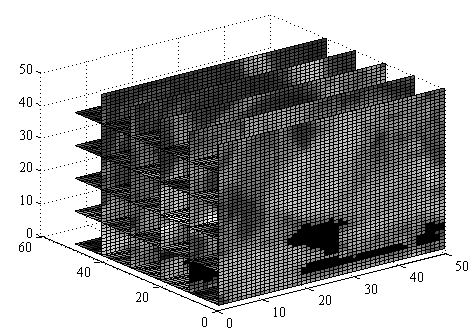
\includegraphics[width=\textwidth]{images/dot_product_image1}
                \subcaption{}
                \label{fig:dot-product-image1}
        \end{subfigure}
        \begin{subfigure}[b]{0.22\textwidth}
                \centering
                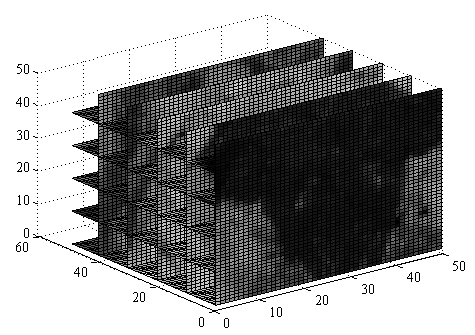
\includegraphics[width=\textwidth]{images/dot_product_image2}
                \subcaption{}
                \label{fig:dot-product-image2}
        \end{subfigure}
        \\ % New Line
        \begin{subfigure}[b]{0.45\textwidth}
                \centering
                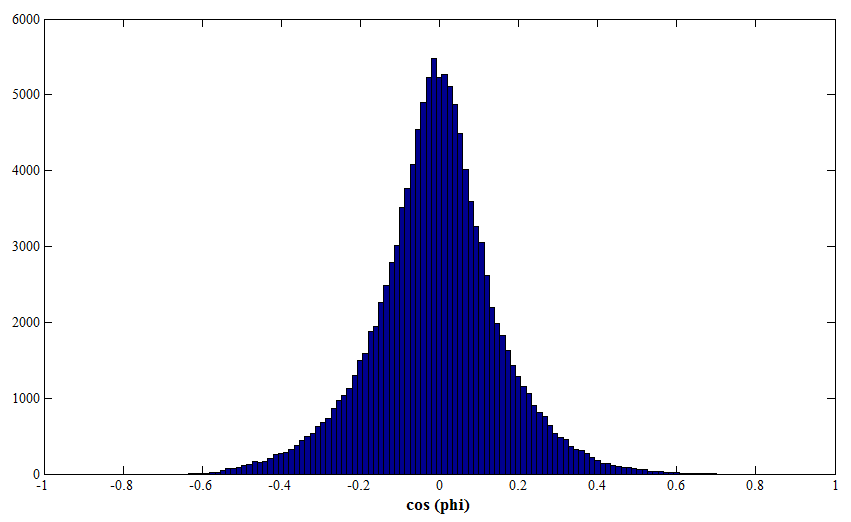
\includegraphics[width=\textwidth]{images/dot_product_hist}
                \subcaption{}
                \label{fig:dot-product-hist}
        \end{subfigure}
        \caption{(a)-(b) Two images use to compare the dot product distribution. The images are visually dissimilar and taken from the Visible Human data-set. The volumes are represented as a series of 2D slices. (c) The distribution of $\cos \phi$ between the two images.}
        \label{fig:dot-product-distribution}
\end{figure}
%%%%%%%%%%%%%%%%%%%%%%%%%%%%%%%%%%%%%%%%%%%%%%%%%%%%%%%%%%%%%%%%%%%%%%%%%%%%%%%%

%%%%%%%%%%%%%%%%%%%%%%%%%%%%%%%%%%%%%%%%%%%%%%%%%%%%%%%%%%%%%%%%%%%%%%%%%%%%%%%%
\subsection{Spherical Correlation}\label{subsec:spherical-corr}
%%%%%%%%%%%%%%%%%%%%%%%%%%%%%%%%%%%%%%%%%%%%%%%%%%%%%%%%%%%%%%%%%%%%%%%%%%%%%%%%
In order to use the robustness properties of \cite{RefWorks:6}, we apply the spherical representation of normals. This allows us to represent the normals in terms of their azimuth and elevation angle. Due to the normalised nature of our gradients, every coordinate lies upon the surface of a unit sphere. The spherical representation is defined by the azimuth angle, $\phi_i \triangleq \arctan [\frac{\tildeg_{i,y}}{\tildeg_{i,x}}]$ and the elevation angle, $\theta_i \triangleq \arccos [\tildeg_{i,z}]$. We can then formulate the correlation as a sum of angle differences
%%%%%%%%%%%%%%%%%%%%%%%%%%%%%%%%%%%%%%%%%%%%%%%%%%%%%%%%%%%%%%%%%%%%%%%%%%%%%%%%
\begin{equation}\label{eq:spherical-cosine}
    s \triangleq \sum_{k \in P} \cos [\Delta \phi (k)] + \sum_{k \in P} \cos [\Delta \theta (k)]
\end{equation}
%%%%%%%%%%%%%%%%%%%%%%%%%%%%%%%%%%%%%%%%%%%%%%%%%%%%%%%%%%%%%%%%%%%%%%%%%%%%%%%%
where $\Delta \phi (k) \triangleq \phi_1 (k) - \phi_2 (k)$ and $\Delta \theta (k) \triangleq \theta_1 (k) - \theta_2 (k)$.

$\phi_i$ is equivalent to gradient orientation in 2D images \cite{RefWorks:6}, hence the difference $\Delta \phi (k)$ between two visually pixel-wise dissimilar images can be assumed to follow $U(0, 2 \pi)$. This was also widely validated in the 3D case through extensive experimentation. Figure~\ref{fig:spherical-distribution} shows the approximate uniform distribution formed by $\Delta \phi$ data from within the Visible Human data set.
%%%%%%%%%%%%%%%%%%%%%%%%%%%%%%%%%%%%%%%%%%%%%%%%%%%%%%%%%%%%%%%%%%%%%%%%%%%%%%%%
\begin{figure}[h!]
        \centering
        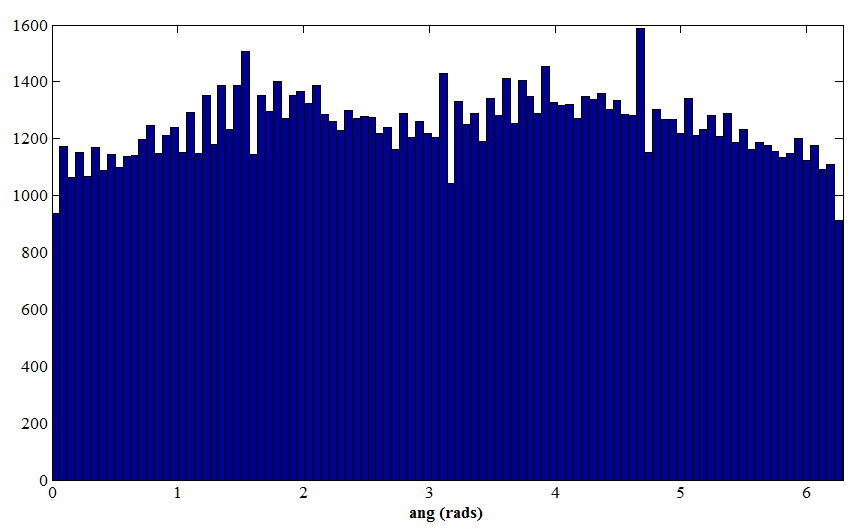
\includegraphics[width=0.45\textwidth]{images/spherical_hist}
        \caption{The distribution of $\Delta \phi$ for the images shown in Figures \ref{fig:dot-product-image1} and \ref{fig:dot-product-image2}}
        \label{fig:spherical-distribution}
\end{figure}
%%%%%%%%%%%%%%%%%%%%%%%%%%%%%%%%%%%%%%%%%%%%%%%%%%%%%%%%%%%%%%%%%%%%%%%%%%%%%%%%

Unfortunately, we cannot apply directly the optimisation procedure proposed in \cite{RefWorks:6} to optimise (\ref{eq:spherical-cosine}) with regards to the parameters, since it is based on the sum of two different cost functions. Nevertheless, we can formulate (\ref{eq:spherical-cosine}) as a least-squares problem, by observing that, since $\cos^2 \alpha + \sin^2 \alpha = 1 \; \forall \alpha$, then maximisation of
%%%%%%%%%%%%%%%%%%%%%%%%%%%%%%%%%%%%%%%%%%%%%%%%%%%%%%%%%%%%%%%%%%%%%%%%%%%%%%%%
\begin{equation}\label{eq:maximise-cos}
   \sum_{k \in P} \cos [\Delta \phi (k)] + \sum_{k \in P} \cos [\Delta \theta (k)]
\end{equation}
%%%%%%%%%%%%%%%%%%%%%%%%%%%%%%%%%%%%%%%%%%%%%%%%%%%%%%%%%%%%%%%%%%%%%%%%%%%%%%%%
is equivalent to the minimisation of
%%%%%%%%%%%%%%%%%%%%%%%%%%%%%%%%%%%%%%%%%%%%%%%%%%%%%%%%%%%%%%%%%%%%%%%%%%%%%%%%
\begin{equation}\label{eq:minimise-least-squares}
       \sum_{k \in P} \Big[ 
        \begin{pmatrix}
            \cos \phi_1 (k) \\ 
            \sin \phi_1 (k) \\
            \cos \theta_1 (k) \\ 
            \sin \theta_1 (k)
        \end{pmatrix}
        -
        \begin{pmatrix}
            \cos \phi_2 (k) \\ 
            \sin \phi_2 (k) \\
            \cos \theta_2 (k) \\ 
            \sin \theta_2 (k)
        \end{pmatrix}
        \Big] ^2
\end{equation}
%%%%%%%%%%%%%%%%%%%%%%%%%%%%%%%%%%%%%%%%%%%%%%%%%%%%%%%%%%%%%%%%%%%%%%%%%%%%%%%%
This least-squares formulation of the correlation can then be easily solved within any least-squares minimisation framework. 

%%%%%%%%%%%%%%%%%%%%%%%%%%%%%%%%%%%%%%%%%%%%%%%%%%%%%%%%%%%%%%%%%%%%%%%%%%%%%%%%
\subsection{Parametric Image Alignment}\label{subsec:parametric-alignment}
%%%%%%%%%%%%%%%%%%%%%%%%%%%%%%%%%%%%%%%%%%%%%%%%%%%%%%%%%%%%%%%%%%%%%%%%%%%%%%%%
Parametric image alignment assumes that $\I_1$ and $\I_2$ are related by a parametric warp
%%%%%%%%%%%%%%%%%%%%%%%%%%%%%%%%%%%%%%%%%%%%%%%%%%%%%%%%%%%%%%%%%%%%%%%%%%%%%%%%
\begin{equation}\label{eq:image-warp}
   I_1 (\boldsymbol{x_k}) = I_2(\W(\boldsymbol{x_k};\p)), \; \forall{k} \in P
\end{equation}
%%%%%%%%%%%%%%%%%%%%%%%%%%%%%%%%%%%%%%%%%%%%%%%%%%%%%%%%%%%%%%%%%%%%%%%%%%%%%%%%
where $\W(\boldsymbol{x_k};\p)$ is a parametric transformation with respect to the unknown parameters $\p = \left[p(1), ..., p(n)\right]^T$ and the image coordinates $\boldsymbol{x_k} = \left[x_1(k) x_2(k)\right]^T$. We can then estimate $\p$ by minimizing an objective function in an iterative fashion by performing a Taylor expansion on either $\I_1$ or $\I_2$. In the following two sections we will show how to optimise (\ref{eq:inner-product-cosine}) and (\ref{eq:spherical-cosine}) with respect to the unknown motion parameters, $\p$.
\section{Optimising The Inner Product Correlation}\label{sec:inner-product}
In this section we focus on how the correlation of (\ref{eq:inner-product-cosine}) can be optimised in order retrieve the motion parameters. The motion parameters, $\p$, can be estimated by maximising
%%%%%%%%%%%%%%%%%%%%%%%%%%%%%%%%%%%%%%%%%%%%%%%%%%%%%%%%%%%%%%%%%%%%%%%%%%%%%%%%
\begin{equation}
  \begin{aligned}\label{eq:eucq}
    q &= \sum \limits_{k \in P} \cos [\phi (k)] \\
      &= \sum \limits_{k \in P} \tildeg_{1,x}(k)\tildeg_{2,x}(k) + \tildeg_{1,y}(k)\tildeg_{2,y}(k) + \tildeg_{1,z}(k)\tildeg_{2,z}(k)
  \end{aligned}
\end{equation}
%%%%%%%%%%%%%%%%%%%%%%%%%%%%%%%%%%%%%%%%%%%%%%%%%%%%%%%%%%%%%%%%%%%%%%%%%%%%%%%%
However, a first order Taylor expansion of either $\tildeg_1$ or $\tildeg_2$ with respect to $\deltap$ results in a linear function of $\deltap$. In order to avoid the computation of the second order Taylor expansion, we take the approach outlined by \cite{RefWorks:59} and normalise the cost function according to $\tildeg_2$. This yields a cost function of the form
%%%%%%%%%%%%%%%%%%%%%%%%%%%%%%%%%%%%%%%%%%%%%%%%%%%%%%%%%%%%%%%%%%%%%%%%%%%%%%%%
\begin{equation}
  \begin{aligned}\label{eq:eucqg2}
    q &= \frac{\sum \limits_{k \in P} \tildeg_{1,x}(k)\tildeg_{2,x}(k) + \tildeg_{1,y}(k)\tildeg_{2,y}(k) + \tildeg_{1,z}(k)\tildeg_{2,z}(k)}{\sqrt{\sum \limits_{k \in P} \tildeg_{2,x}^2(k) + \tildeg_{2,y}^2(k) + \tildeg_{2,z}^2(k)}} \\
      &= \frac{\tildeg_{1,x}^T \tildeg_{2,x} + \tildeg_{1,y}^T \tildeg_{2,y} + \tildeg_{1,z}^T \tildeg_{2,z}}{\sqrt{\tildeg_{2,x}^T \tildeg_{2,x} + \tildeg_{2,y}^T \tildeg_{2,y} + \tildeg_{2,z}^T \tildeg_{2,z}}}
  \end{aligned}
\end{equation}
%%%%%%%%%%%%%%%%%%%%%%%%%%%%%%%%%%%%%%%%%%%%%%%%%%%%%%%%%%%%%%%%%%%%%%%%%%%%%%%%
where, if we linearize $\tildeg_2$, we have a non-linear function of $\deltap$. We can then maximise $q$ with respect to $\p$ by assuming a current estimate of $\p$ is known and looking for an increment $\deltap$ that maximises (\ref{eq:eucqg2}).
%%%%%%%%%%%%%%%%%%%%%%%%%%%%%%%%%%%%%%%%%%%%%%%%%%%%%%%%%%%%%%%%%%%%%%%%%%%%%%%%
\subsection{The inner product inverse-compositional gradient correlation algorithm}\label{subsec:3deucinvcomp}
We choose to provide the derivation of the inverse-compositional form of the algorithm, due to the pre-computable nature of the Hessian in this form. However, a forward-additive version of the algorithm would be simple to implement following a similar logic.

For the inverse-compositional algorithm, we swap the roles of $\I_1$ and $\I_2$ and the cost function is defined as
%%%%%%%%%%%%%%%%%%%%%%%%%%%%%%%%%%%%%%%%%%%%%%%%%%%%%%%%%%%%%%%%%%%%%%%%%%%%%%%%
% WITH NOTATION
%\begin{equation}\label{eq:eucinvcomp}
%    q = \frac{(\tildeg_{2,x}[p])^T (\tildeg_{1,x}[\deltap])+ (\tildeg_{2,y}[p])^T (\tildeg_{1,y}[\deltap]) + (\tildeg_{2,z}[p])^T (\tildeg_{1,z}[\deltap])}{\sqrt{(\tildeg_{1,x}[\deltap])^T (\tildeg_{1,x}[\deltap]) +(\tildeg_{1,y}[\deltap])^T (\tildeg_{1,y}[\deltap]) + (\tildeg_{1,z}[\deltap])^T (\tildeg_{1,z}[\deltap])}}
%\end{equation}
%%%%%%%%%%%%%%%%%%%%%%%%%%%%%%%%%%%%%%%%%%%%%%%%%%%%%%%%%%%%%%%%%%%%%%%%%%%%%%%%%
%%%%%%%%%%%%%%%%%%%%%%%%%%%%%%%%%%%%%%%%%%%%%%%%%%%%%%%%%%%%%%%%%%%%%%%%%%%%%%%%
\begin{equation}\label{eq:eucinvcomp}
    q = \frac{\tildeg_{2,x}^T \tildeg_{1,x} + \tildeg_{2,y}^T \tildeg_{1,y} + \tildeg_{2,z}^T \tildeg_{1,z}}{\sqrt{\tildeg_{1,x}^T \tildeg_{1,x} + \tildeg_{1,y}^T \tildeg_{1,y} + \tildeg_{1,z}^T \tildeg_{1,z})}}
\end{equation}
%%%%%%%%%%%%%%%%%%%%%%%%%%%%%%%%%%%%%%%%%%%%%%%%%%%%%%%%%%%%%%%%%%%%%%%%%%%%%%%%%
where $\tildeg_1$ has a dependency on $\deltap$ and $\tildeg_2$ has a dependency on $\p$, which have been omitted for notational simplicity.

$\I_2$ is then updated at each iteration using the compositional update $\W(\x;\p) \leftarrow \W(\x;\p) \circ (\W(\x;\p))^{-1}$. It is also assumed that $\W(\x;\zero) = \x$ and thus the Taylor expansion is performed around zero. The derivation is split in to separate entities for each dimension, $x$, $y$ and $z$. The first Taylor expansion on $\tildeg_{1,x}[\p + \deltap]$ produces
%%%%%%%%%%%%%%%%%%%%%%%%%%%%%%%%%%%%%%%%%%%%%%%%%%%%%%%%%%%%%%%%%%%%%%%%%%%%%%%%
\begin{equation}\label{eq:eucgx}
    \tildeg_{1,x}[\deltap] \approx \tildeg_{1,x}[\zero] + \nabla \tildeg_{1,x}[\zero] \deltap
\end{equation}
%%%%%%%%%%%%%%%%%%%%%%%%%%%%%%%%%%%%%%%%%%%%%%%%%%%%%%%%%%%%%%%%%%%%%%%%%%%%%%%%
By the chain rule we can decompose $\nabla \tildeg_{1,x}[\zero]$ in to
%%%%%%%%%%%%%%%%%%%%%%%%%%%%%%%%%%%%%%%%%%%%%%%%%%%%%%%%%%%%%%%%%%%%%%%%%%%%%%%%
\begin{equation}
  \begin{aligned}\label{eq:nablagx}
    \nabla \tildeg_{1,x}[\zero] &= \frac{\partial \tildeg_{1,x}[\p]}{\partial \p}\Big|_{p=0} \\
                              &= \frac{\partial f(\g_{1,x}[\p])}{\partial \g_{1,x}[\p]} \; \frac{\partial \g_{1,x}[\p]}{\partial \p}\Big|_{\p=0}
  \end{aligned}
\end{equation}
%%%%%%%%%%%%%%%%%%%%%%%%%%%%%%%%%%%%%%%%%%%%%%%%%%%%%%%%%%%%%%%%%%%%%%%%%%%%%%%%
We provide the derivation for (\ref{eq:nablagx}) as follows:
%%%%%%%%%%%%%%%%%%%%%%%%%%%%%%%%%%%%%%%%%%%%%%%%%%%%%%%%%%%%%%%%%%%%%%%%%%%%%%%%
\begin{equation}
  \begin{aligned}\label{eq:derivefgx}
    \frac{\partial f(\g_{1,x}[\p])}{\partial \g_{1,x}[\p]}\Big|_{\p=0} &= \frac{\partial \frac{\g_{1,x}[\p]}{\sqrt{\g_{1,x}^2[\p] + \g_{1,y}^2[\p] + \g_{1,z}^2[\p]}}}{\partial \g_{1,x}[\p]}\Bigg|_{\p=0} \\
     &= \frac{\g_{1,y}^2[\zero] + \g_{1,z}[\zero]^2}{(\g_{1,x}^2[\zero] + \g_{1,y}^2[\zero] + \g_{1,z}^2[\zero])^{3/2}}
  \end{aligned}
\end{equation}
%%%%%%%%%%%%%%%%%%%%%%%%%%%%%%%%%%%%%%%%%%%%%%%%%%%%%%%%%%%%%%%%%%%%%%%%%%%%%%%%
%%%%%%%%%%%%%%%%%%%%%%%%%%%%%%%%%%%%%%%%%%%%%%%%%%%%%%%%%%%%%%%%%%%%%%%%%%%%%%%%
\begin{equation}\label{eq:derivegxp}
    \frac{\partial \g_{1,x}[\p]}{\partial \p}\Big|_{\p=0} = [ \g_{1,xx}[\zero](k) \; \g_{1,xy}[\zero](k) \; \g_{1,xz}[\zero](k) ] \frac{\partial \W}{\partial \p}
\end{equation}
%%%%%%%%%%%%%%%%%%%%%%%%%%%%%%%%%%%%%%%%%%%%%%%%%%%%%%%%%%%%%%%%%%%%%%%%%%%%%%%%%
Where the result from (\ref{eq:derivegxp}) is as described by Equation (12) of \cite{RefWorks:6}. To simplify the expressions, we define a function $f(a,b)$, such that
%%%%%%%%%%%%%%%%%%%%%%%%%%%%%%%%%%%%%%%%%%%%%%%%%%%%%%%%%%%%%%%%%%%%%%%%%%%%%%%%
\begin{equation}\label{eq:f-simplify}
    f(a,b) = \frac{\g_{1,a}^2 + \g_{1,b}^2}{(\g_{1,x}^2 + \g_{1,y}^2 + \g_{1,z}^2)^{3/2}}
\end{equation}
%%%%%%%%%%%%%%%%%%%%%%%%%%%%%%%%%%%%%%%%%%%%%%%%%%%%%%%%%%%%%%%%%%%%%%%%%%%%%%%%%
Therefore, we define $\tildeg_{1,x}[\deltap]$, $\tildeg_{1,y}[\deltap]$ and $\tildeg_{1,z}[\deltap]$ as
%%%%%%%%%%%%%%%%%%%%%%%%%%%%%%%%%%%%%%%%%%%%%%%%%%%%%%%%%%%%%%%%%%%%%%%%%%%%%%%%
\begin{equation}
  \begin{aligned}\label{eq:eucgyz}
    \tildeg_{1,x}[\deltap] &\approx \tildeg_{1,x}[\zero] + f(y,z)[\zero] \; \nabla \g_{1,x}[\zero] \frac{\partial \W}{\partial \p} \deltap \\  
    \tildeg_{1,y}[\deltap] &\approx \tildeg_{1,y}[\zero] + f(x,z)[\zero] \; \nabla \g_{1,y}[\zero] \frac{\partial \W}{\partial \p} \deltap \\
    \tildeg_{1,z}[\deltap] &\approx \tildeg_{1,z}[\zero] + f(x,y)[\zero] \; \nabla \g_{1,z}[\zero] \frac{\partial \W}{\partial \p} \deltap
  \end{aligned}
\end{equation}
%%%%%%%%%%%%%%%%%%%%%%%%%%%%%%%%%%%%%%%%%%%%%%%%%%%%%%%%%%%%%%%%%%%%%%%%%%%%%%%%
 and
%%%%%%%%%%%%%%%%%%%%%%%%%%%%%%%%%%%%%%%%%%%%%%%%%%%%%%%%%%%%%%%%%%%%%%%%%%%%%%%%
\begin{equation}
  \begin{aligned}\label{eq:euc-second-order-derivs}
    \nabla \g_{1,x}[\zero] &= [ \g_{1,xx}[\zero](k) \; \g_{1,xy}[\zero](k) \; \g_{1,xz}[\zero](k) ] \\
    \nabla \g_{1,y}[\zero] &= [ \g_{1,yx}[\zero](k) \; \g_{1,yy}[\zero](k) \; \g_{1,yz}[\zero](k) ] \\
    \nabla \g_{1,z}[\zero] &= [ \g_{1,zx}[\zero](k) \; \g_{1,zy}[\zero](k) \; \g_{1,zz}[\zero](k) ]
  \end{aligned}
\end{equation}
%%%%%%%%%%%%%%%%%%%%%%%%%%%%%%%%%%%%%%%%%%%%%%%%%%%%%%%%%%%%%%%%%%%%%%%%%%%%%%%%

Equations (\ref{eq:eucgyz}) and (\ref{eq:eucgx}) can be plugged in to (\ref{eq:eucqg2}) to arrive at the cost function $q(\deltap)$. In the formulae below, the dependencies on $[\zero]$ and $[\deltap]$ are dropped for notational simplicity. The numerator is as follows
%%%%%%%%%%%%%%%%%%%%%%%%%%%%%%%%%%%%%%%%%%%%%%%%%%%%%%%%%%%%%%%%%%%%%%%%%%%%%%%%
\begin{equation}
  \begin{aligned}\label{eq:q_dp_num}
    q(\deltap) &= \tildeg_{2,x}^T (\tildeg_{1,x} + \nabla \tildeg_{1,x} \deltap) + \tildeg_{2,y}^T (\tildeg_{1,y} + \nabla \tildeg_{1,y} \deltap) \\
    & \hspace{4 mm} + \tildeg_{2,z}^T (\tildeg_{1,z} + \nabla \tildeg_{1,z} \deltap) \\
    &= \tildeg_{2,x}^T \tildeg_{1,x} + \tildeg_{2,y}^T \tildeg_{1,y} + \tildeg_{2,z}^T \tildeg_{1,z} \\     
    & \hspace{4 mm} + \left( \tildeg_{2,x}^T \nabla \tildeg_{1,x} + \tildeg_{2,y}^T \nabla \tildeg_{1,y} + \tildeg_{2,z}^T \nabla \tildeg_{1,z} \right) \deltap \\
    %&= [\tildeg_{2,x} \; \tildeg_{2,y} \; \tildeg_{2,z}]^T [\tildeg_{1,x} \; \tildeg_{1,y} \; \tildeg_{1,z}] + [\tildeg_{2,x} \; \tildeg_{2,y} \; \tildeg_{2,z}]^T [\nabla \tildeg_{1,x} \; \nabla \tildeg_{1,y} \; \nabla \tildeg_{1,z}] \deltap \\
    &= q_p + \GTwo^T \J \deltap
  \end{aligned}
\end{equation}
%%%%%%%%%%%%%%%%%%%%%%%%%%%%%%%%%%%%%%%%%%%%%%%%%%%%%%%%%%%%%%%%%%%%%%%%%%%%%%%%
where $\J = \left[ \nabla \tildeg_{2,x} \; \nabla \tildeg_{2,y} \; \nabla \tildeg_{2,z} \right]^T$ as described in (\ref{eq:nablagx})-(\ref{eq:derivegxp}) and $\GTwo = \left[ \tildeg_{2,x} \; \tildeg_{2,y} \; \tildeg_{2,z} \right]^T$. The denominator is defined as
\begin{equation}
  \begin{aligned}\label{eq:q_dp_denom}
    q(\deltap) &= \left( (\tildeg_{1,x} + \nabla \tildeg_{1,x} \deltap)^T (\tildeg_{1,x} + \nabla \tildeg_{1,x} \deltap) + \right. \\
    & \hspace{6 mm} \left. (\tildeg_{1,y} + \nabla \tildeg_{1,y} \deltap)^T (\tildeg_{1,y} + \nabla \tildeg_{1,y} \deltap) + \right. \\
    & \hspace{5 mm} \left. (\tildeg_{1,z} + \nabla \tildeg_{1,z} \deltap)^T (\tildeg_{1,z} + \nabla \tildeg_{1,z} \deltap) \right)^{1/2} \\
    %&= \left( \sum_k (\tildeg_{1,x} + \nabla \tildeg_{1,x} \deltap)^2 + (\tildeg_{1,y} + \nabla \tildeg_{1,y} \deltap)^2 + \\
    %& \hspace{12 mm} (\tildeg_{1,z} + \nabla \tildeg_{1,z} \deltap)^2 \right)^{1/2} \\
    &= \left( \sum_k \tildeg^2_{1,x} + \tildeg^2_{1,y} + \tildeg^2_{1,z} + 2 \; \tildeg_{1,x} \nabla \tildeg_{1,x} \deltap + \right. \\
    & \hspace{4 mm} \left. 2 \; \tildeg_{1,y} \nabla \tildeg_{1,y} \deltap + 2 \; \tildeg_{1,z} \nabla \tildeg_{1,z} \deltap + \right. \\
    & \hspace{4 mm} \left. \vphantom{\sum_k} (\nabla \tildeg_{1,x} \deltap)^2 + (\nabla \tildeg_{1,y} \deltap)^2 +(\nabla \tildeg_{1,z} \deltap)^2 \right)^{1/2} \\
    &= \sqrt{\norm{\GOne}^2 + 2 \GOne^T \J \deltap + \deltap^T \J^T \J \deltap}
  \end{aligned}
\end{equation}
%%%%%%%%%%%%%%%%%%%%%%%%%%%%%%%%%%%%%%%%%%%%%%%%%%%%%%%%%%%%%%%%%%%%%%%%%%%%%%%%
We can then combine (\ref{eq:q_dp_num}) and (\ref{eq:q_dp_denom}) together to form the cost function
%%%%%%%%%%%%%%%%%%%%%%%%%%%%%%%%%%%%%%%%%%%%%%%%%%%%%%%%%%%%%%%%%%%%%%%%%%%%%%%%
\begin{equation}\label{eq:q_dp}
    q(\deltap) = \frac{q_p + \GTwo^T \J \deltap}{\sqrt{\norm{\GOne}^2 + 2 \GOne^T \J \deltap + \deltap^T \J^T \J \deltap}}
\end{equation}
%%%%%%%%%%%%%%%%%%%%%%%%%%%%%%%%%%%%%%%%%%%%%%%%%%%%%%%%%%%%%%%%%%%%%%%%%%%%%%%%
where $\GOne = \left[ \tildeg_{1,x} \; \tildeg_{1,y} \; \tildeg_{1,z} \right]^T$. Finally, we maximise (\ref{eq:q_dp}) as in \cite{RefWorks:59} We first note that we have a cost function of the form
%%%%%%%%%%%%%%%%%%%%%%%%%%%%%%%%%%%%%%%%%%%%%%%%%%%%%%%%%%%%%%%%%%%%%%%%%%%%%%%%
\begin{equation*}
    f(x) = \frac{u + \boldsymbol{u}\boldsymbol{x}}{\sqrt{v + 2 \boldsymbol{v}^T \boldsymbol{x} + \boldsymbol{x}^T  \boldsymbol{Q} \boldsymbol{x}}}
\end{equation*}
%%%%%%%%%%%%%%%%%%%%%%%%%%%%%%%%%%%%%%%%%%%%%%%%%%%%%%%%%%%%%%%%%%%%%%%%%%%%%%%%
and we can therefore derive two different maxima. 

\textbf{(Case 1)} $u > \boldsymbol{u}^T \boldsymbol{Q}^{-1} \boldsymbol{v}$: Here we have a maximum of $x$ which is attainable from the equation
%%%%%%%%%%%%%%%%%%%%%%%%%%%%%%%%%%%%%%%%%%%%%%%%%%%%%%%%%%%%%%%%%%%%%%%%%%%%%%%%
\begin{equation}\label{eq:case1}
    x = \boldsymbol{Q}^{-1} \left( \frac{v - \boldsymbol{v}^T  \boldsymbol{Q}^{-1} \boldsymbol{v}}{u - \boldsymbol{u}^T \boldsymbol{Q}^{-1} \boldsymbol{v}} \boldsymbol{u} - \boldsymbol{v} \right)
\end{equation}
%%%%%%%%%%%%%%%%%%%%%%%%%%%%%%%%%%%%%%%%%%%%%%%%%%%%%%%%%%%%%%%%%%%%%%%%%%%%%%%%
\textbf{(Case 2)} $u \le \boldsymbol{u}^T \boldsymbol{Q}^{-1} \boldsymbol{v}$ : Here we have a maximum of $x$ which is attainable from the equation
%%%%%%%%%%%%%%%%%%%%%%%%%%%%%%%%%%%%%%%%%%%%%%%%%%%%%%%%%%%%%%%%%%%%%%%%%%%%%%%%
\begin{equation}\label{eq:case2}
    x = \boldsymbol{Q}^{-1} \left( \lambda \boldsymbol{u} - \boldsymbol{v} \right)
\end{equation}
%%%%%%%%%%%%%%%%%%%%%%%%%%%%%%%%%%%%%%%%%%%%%%%%%%%%%%%%%%%%%%%%%%%%%%%%%%%%%%%%
where $\lambda$ can have the possible values of
%%%%%%%%%%%%%%%%%%%%%%%%%%%%%%%%%%%%%%%%%%%%%%%%%%%%%%%%%%%%%%%%%%%%%%%%%%%%%%%%
\begin{equation}\label{eq:lambda}
    \lambda_1 = \sqrt{\frac{\boldsymbol{v}^T \boldsymbol{Q}^{-1} \boldsymbol{v}}{\boldsymbol{u}^T \boldsymbol{Q}^{-1} \boldsymbol{u}}} \qquad \lambda_2 = \frac{\boldsymbol{u}^T \boldsymbol{Q}^{-1} \boldsymbol{v} - \boldsymbol{u}^T \boldsymbol{v}}{\boldsymbol{u}^T \boldsymbol{Q}^{-1} \boldsymbol{u}}
\end{equation}
%%%%%%%%%%%%%%%%%%%%%%%%%%%%%%%%%%%%%%%%%%%%%%%%%%%%%%%%%%%%%%%%%%%%%%%%%%%%%%%%
Equation~(\ref{eq:case2}) should only be used when the denominator is negative and thus we are not close to the optimum solution. In this case we are unlikely to ever reach the optimum value and so we choose to use Equation~(\ref{eq:case1}) to calculate our maximum. Through matching of terms between (\ref{eq:case1}) and (\ref{eq:q_dp}) we arrive at
%%%%%%%%%%%%%%%%%%%%%%%%%%%%%%%%%%%%%%%%%%%%%%%%%%%%%%%%%%%%%%%%%%%%%%%%%%%%%%%%
\begin{equation}\label{eq:max_deltap}
    \deltap = (\J^T \J)^{-1} \J^T \left( \frac{\norm{\GOne}^2 - \GOne^T \boldsymbol{P_G} \GOne}{\GTwo^T \GOne - \GTwo^T \boldsymbol{P_G} \GOne} \GTwo - \GOne \right)
\end{equation}
%%%%%%%%%%%%%%%%%%%%%%%%%%%%%%%%%%%%%%%%%%%%%%%%%%%%%%%%%%%%%%%%%%%%%%%%%%%%%%%%
where $\boldsymbol{P_G} \triangleq \J (\J^T \J)^{-1} \J^T$ and $\boldsymbol{P_G}$ is an orthogonal projection operator.
\section{Optimising The Spherical Correlation}\label{sec:spherical}
%%%%%%%%%%%%%%%%%%%%%%%%%%%%%%%%%%%%%%%%%%%%%%%%%%%%%%%%%%%%%%%%%%%%%%%%%%%%%%%%
In this section we show how (\ref{eq:minimise-least-squares}) can be optimised with respect to the motion parameters. As described in Subsection~\ref{subsec:spherical-corr}, we define two angles to represent our gradient orientation. These angles are described as  $\phi \triangleq \arctan \frac{\tildeg_y}{\tildeg_x}$, the azimuth angle, and the elevation angle, denoted by $\theta \triangleq \arccos \tildeg_z$. Given these relationships, we can define the least-squares minimization problem
%%%%%%%%%%%%%%%%%%%%%%%%%%%%%%%%%%%%%%%%%%%%%%%%%%%%%%%%%%%%%%%%%%%%%%%%%%%%%%%%
\begin{equation}
  \begin{aligned}\label{eq:ang-least-squares}
    &  \argmax \sum_{k \in P} \cos [\Delta \phi (k)] + \sum_{k \in P} \cos [\Delta \theta (k)] \\
    &\triangleq \argmin \sum_{k \in P} \Big[ 
        \begin{pmatrix}
            \cos{\phi_1} \\
            \sin{\phi_1} \\
            \cos{\theta_1} \\
            \sin{\theta_1}
        \end{pmatrix}
        -
        \begin{pmatrix}
            \cos{\phi_2} \\
            \sin{\phi_2} \\
            \cos{\theta_2} \\
            \sin{\theta_2}
        \end{pmatrix}
        \Big] ^2 \\
    &\triangleq \argmin \sum_{k \in P} \Big[ 
        \begin{pmatrix}
            \tildeg_{1,x} \\ 
            \tildeg_{1,y} \\ 
            \tildeg_{1,z} \\ 
            \sqrt{1 - \tildeg_{1,z}^2}
        \end{pmatrix}
        -
        \begin{pmatrix}
            \tildeg_{2,x} \\ 
            \tildeg_{2,y} \\ 
            \tildeg_{2,z} \\ 
            \sqrt{1 - \tildeg_{2,z}^2}
        \end{pmatrix}
        \Big] ^2
    \end{aligned}
\end{equation}
%%%%%%%%%%%%%%%%%%%%%%%%%%%%%%%%%%%%%%%%%%%%%%%%%%%%%%%%%%%%%%%%%%%%%%%%%%%%%%%%
\subsection{The spherical inverse-compositional gradient correlation algorithm}\label{subsec:3danginvcomp}
For the spherical inverse-compositional algorithm, we swap the roles of $\I_1$ and $\I_2$ and formulate the least-squares problem described in (\ref{eq:ang-least-squares})
%%%%%%%%%%%%%%%%%%%%%%%%%%%%%%%%%%%%%%%%%%%%%%%%%%%%%%%%%%%%%%%%%%%%%%%%%%%%%%%%
\begin{equation}\label{eq:ang-minimization}
    \sum_{k \in P} \Big[ 
        \begin{pmatrix}
            \tildeg_{2,x}[\p] \\ 
            \tildeg_{2,y}[\p] \\ 
            \tildeg_{2,z}[\p] \\ 
            \sqrt{1 - \tildeg_{2,z}^2[\p]}
        \end{pmatrix}
        -
        \begin{pmatrix}
            \tildeg_{1,x}[\deltap] \\ 
            \tildeg_{1,y}[\deltap] \\ 
            \tildeg_{1,z}[\deltap] \\ 
            \sqrt{1 - \tildeg_{1,z}^2[\deltap]}
        \end{pmatrix}
        \Big] ^2
\end{equation}
%%%%%%%%%%%%%%%%%%%%%%%%%%%%%%%%%%%%%%%%%%%%%%%%%%%%%%%%%%%%%%%%%%%%%%%%%%%%%%%%
$\I_2$ is then updated at each iteration using $\W(\x;\p) \leftarrow \W(\x;\p) \circ (\W(\x;\p))^{-1}$ where $\circ$ signifies composition. The derivation of the first Taylor expansion of (\ref{eq:ang-minimization}) is very similar to that of (\ref{eq:eucgyz}). Therefore, after applying the first Taylor expansion to each term and expanding the chain rule as in (\ref{eq:nablagx}), we arrive at
%%%%%%%%%%%%%%%%%%%%%%%%%%%%%%%%%%%%%%%%%%%%%%%%%%%%%%%%%%%%%%%%%%%%%%%%%%%%%%%%
\begin{equation}
  \begin{aligned}\label{eq:anggxyz}
    &\tildeg_{1,x}[\deltap] \approx \tildeg_{1,x}[\zero] + \nabla_g (\g_{1,x}[\zero]) \nabla_p (\g_{1,x}[\zero]) \frac{\partial \W}{\partial \p} \deltap \\  
    &\tildeg_{1,y}[\deltap] \approx \tildeg_{1,y}[\zero] + \nabla_g (\g_{1,y}[\zero]) \nabla_p (\g_{1,y}[\zero]) \frac{\partial \W}{\partial \p} \deltap \\
    &\tildeg_{1,z}[\deltap] \approx \tildeg_{1,z}[\zero] + \nabla_g (\g_{1,z}[\zero]) \nabla_p (\g_{1,z}[\zero])  \frac{\partial \W}{\partial \p} \deltap \\
    &\sqrt{1 - \tildeg_{1,z}^2[\deltap]} \approx \sqrt{1 - \tildeg_{1,z}^2[\zero]} + \\
    & \hspace{30 mm} \nabla_g (\g_{1,sz}[\zero]) \nabla_p (\g_{1,z}[\zero])  \frac{\partial \W}{\partial \p} \deltap
  \end{aligned}
\end{equation}
%%%%%%%%%%%%%%%%%%%%%%%%%%%%%%%%%%%%%%%%%%%%%%%%%%%%%%%%%%%%%%%%%%%%%%%%%%%%%%%%
where
%%%%%%%%%%%%%%%%%%%%%%%%%%%%%%%%%%%%%%%%%%%%%%%%%%%%%%%%%%%%%%%%%%%%%%%%%%%%%%%%
\begin{equation}
  \begin{aligned}\label{eq:spherical-chain-rule}
    \nabla_g (\g_{1,x}[\zero]) &= \frac{\g_{1,y}^2[\zero]}{(\g_{1,x}^2[\zero] + \g_{1,y}^2[\zero] + \g_{1,z}^2[\zero])^{3/2}} \\
    \nabla_g (\g_{1,y}[\zero]) &= \frac{\g_{1,x}^2[\zero]}{(\g_{1,x}^2[\zero] + \g_{1,y}^2[\zero] + \g_{1,z}^2[\zero])^{3/2}} \\
    \nabla_g (\g_{1,z}[\zero]) &= \frac{\g_{1,x}^2[\zero] + \g_{1,y}^2[\zero]}{(\g_{1,x}^2[\zero] + \g_{1,y}^2[\zero] + \g_{1,z}^2[\zero])^{3/2}} \\
    \nabla_g (\g_{1,sz}[\zero]) &= \frac{-(\g_{1,x}[\zero] ( \frac{\g_{1,y}^2[\zero] + \g_{1,z}^2[\zero]}{\g_{1,x}^2[\zero] + \g_{1,y}^2[\zero] + \g_{1,z}^2[\zero]})^{3/2})}{\g_{1,y}^2[\zero] + \g_{1,z}^2[\zero]}
  \end{aligned}
\end{equation}
%%%%%%%%%%%%%%%%%%%%%%%%%%%%%%%%%%%%%%%%%%%%%%%%%%%%%%%%%%%%%%%%%%%%%%%%%%%%%%%%
and
%%%%%%%%%%%%%%%%%%%%%%%%%%%%%%%%%%%%%%%%%%%%%%%%%%%%%%%%%%%%%%%%%%%%%%%%%%%%%%%%
\begin{equation}
  \begin{aligned}\label{eq:spherical-second-order-derivs}
    \nabla_p (\g_{1,x}[\zero]) &= [ \g_{1,xx}[\zero](k) \; \g_{1,xy}[\zero](k) \; \g_{1,xz}[\zero](k) ] \\
    \nabla_p (\g_{1,y}[\zero]) &= [ \g_{1,yx}[\zero](k) \; \g_{1,yy}[\zero](k) \; \g_{1,yz}[\zero](k) ] \\
    \nabla_p (\g_{1,z}[\zero]) &= [ \g_{1,zx}[\zero](k) \; \g_{1,zy}[\zero](k) \; \g_{1,zz}[\zero](k) ] \\
  \end{aligned}
\end{equation}
%%%%%%%%%%%%%%%%%%%%%%%%%%%%%%%%%%%%%%%%%%%%%%%%%%%%%%%%%%%%%%%%%%%%%%%%%%%%%%%%

We can then solve the least squares problem from (\ref{eq:ang-minimization}) in terms of $\deltap$. We first define $\nabla \GOne$ as the vector
%%%%%%%%%%%%%%%%%%%%%%%%%%%%%%%%%%%%%%%%%%%%%%%%%%%%%%%%%%%%%%%%%%%%%%%%%%%%%%%%
\begin{equation}\label{eq:spherical-nabla-g1}
    \nabla \GOne = \begin{pmatrix}
                         \nabla_g (\g_{1,x}[\zero]) \nabla_p (\g_{1,x}[\zero]) \\
                         \nabla_g (\g_{1,y}[\zero]) \nabla_p (\g_{1,y}[\zero]) \\
                         \nabla_g (\g_{1,z}[\zero]) \nabla_p (\g_{1,z}[\zero]) \\
                         \nabla_g (\g_{1,z}[\zero]) \nabla_p (\g_{1,sz}[\zero])
                    \end{pmatrix}
\end{equation}
%%%%%%%%%%%%%%%%%%%%%%%%%%%%%%%%%%%%%%%%%%%%%%%%%%%%%%%%%%%%%%%%%%%%%%%%%%%%%%%%
and $\GOne$ and $\GTwo$ as the the corresponding parts of the residual defined in (\ref{eq:ang-minimization}). Performing a first order Taylor expansion to (\ref{eq:ang-minimization}) gives
%%%%%%%%%%%%%%%%%%%%%%%%%%%%%%%%%%%%%%%%%%%%%%%%%%%%%%%%%%%%%%%%%%%%%%%%%%%%%%%%
\begin{equation}\label{eq:spherical-first-order-expansion}
    \sum_{k \in P} \Big[ \GTwo(k) + \nabla \GOne \frac{\partial \W}{\partial \p} \Delta \p - \GOne(k) \Big]^2
\end{equation}
%%%%%%%%%%%%%%%%%%%%%%%%%%%%%%%%%%%%%%%%%%%%%%%%%%%%%%%%%%%%%%%%%%%%%%%%%%%%%%%%
We can then rearrange (\ref{eq:spherical-first-order-expansion}) to form the equation
%%%%%%%%%%%%%%%%%%%%%%%%%%%%%%%%%%%%%%%%%%%%%%%%%%%%%%%%%%%%%%%%%%%%%%%%%%%%%%%%
\begin{equation}\label{eq:spherical-delta-p}
    \deltap = \boldsymbol{H}^{-1} \sum_k \Big[ \nabla \GOne \frac{\partial \W}{\partial \p} \Big]^T [\GTwo(k) - \GOne(k)]
\end{equation}
%%%%%%%%%%%%%%%%%%%%%%%%%%%%%%%%%%%%%%%%%%%%%%%%%%%%%%%%%%%%%%%%%%%%%%%%%%%%%%%%
where $\boldsymbol{H}$ is the Hessian matrix defined by
%%%%%%%%%%%%%%%%%%%%%%%%%%%%%%%%%%%%%%%%%%%%%%%%%%%%%%%%%%%%%%%%%%%%%%%%%%%%%%%%
\begin{equation}\label{eq:spherical-hessian}
    \boldsymbol{H} = \sum_k \Big[ \nabla \GOne \frac{\partial \W}{\partial \p} \Big]^T \Big[ \nabla \GOne \frac{\partial \W}{\partial \p} \Big]
\end{equation}
%%%%%%%%%%%%%%%%%%%%%%%%%%%%%%%%%%%%%%%%%%%%%%%%%%%%%%%%%%%%%%%%%%%%%%%%%%%%%%%%
\def\kdeltak{k + \Delta k_x}
\newcommand{\IPartial}[1]{\frac{\partial I(k)}{\partial #1}}
\newcommand{\BPartialM}[1]{B(k) \frac{\partial M (k)}{\partial #1}}
\newcommand{\PartialM}[1]{\frac{\partial M (k)}{\partial #1}}

\section{Robustness Against Bias Fields}\label{sec:robustness}
%%%%%%%%%%%%%%%%%%%%%%%%%%%%%%%%%%%%%%%%%%%%%%%%%%%%%%%%%%%%%%%%%%%%%%%%%%%%%%%%
In this section we provide a formal proof of the robustness of our cost functions to bias field corruption. Consider an image signal $M$ with no intensity inhomogeneities and a smooth signal $B$, representing a multiplicative bias field. We assume $B$ to be constant within a small neighbourhood, $N(k) = \left( \Delta k_x \Delta k_y \Delta k_z \right)$. Therefore, for $\Delta k_x$, we have
%%%%%%%%%%%%%%%%%%%%%%%%%%%%%%%%%%%%%%%%%%%%%%%%%%%%%%%%%%%%%%%%%%%%%%%%%%%%%%%%
\begin{equation}
    \begin{aligned}\label{eq:robust-I}
        I(k) &= M(k) B(k) \\
        I(\kdeltak) &= M(\kdeltak) B(\kdeltak)
    \end{aligned}
\end{equation}
%%%%%%%%%%%%%%%%%%%%%%%%%%%%%%%%%%%%%%%%%%%%%%%%%%%%%%%%%%%%%%%%%%%%%%%%%%%%%%%%
and given that $B$ is constant within $N$
%%%%%%%%%%%%%%%%%%%%%%%%%%%%%%%%%%%%%%%%%%%%%%%%%%%%%%%%%%%%%%%%%%%%%%%%%%%%%%%%
\begin{equation}
    \begin{aligned}\label{eq:robust-dIdx}
        \frac{\partial I(k)}{\partial x} &\approx \lim_{\Delta k_x \to 0} \frac{I(\kdeltak) - I(k)}{\Delta k} \\
        &\approx \lim_{\Delta k_x \to 0} \frac{B(k) (M(\kdeltak) - M(k))}{\Delta k} \\
        &= B(k) \frac{\partial M(k)}{\partial x}
    \end{aligned}
\end{equation}
%%%%%%%%%%%%%%%%%%%%%%%%%%%%%%%%%%%%%%%%%%%%%%%%%%%%%%%%%%%%%%%%%%%%%%%%%%%%%%%%
Using (\ref{eq:robust-dIdx}), we show our proposed cost function to be robust to locally constant bias fields, since
%%%%%%%%%%%%%%%%%%%%%%%%%%%%%%%%%%%%%%%%%%%%%%%%%%%%%%%%%%%%%%%%%%%%%%%%%%%%%%%%
\begin{equation}
    \begin{aligned}\label{eq:robust-cost-function}
        &\frac{\IPartial{x}}{\sqrt{(\IPartial{x})^2 + (\IPartial{y})^2 + (\IPartial{y})^2}} \\
        &\approx \frac{\BPartialM{x}}{\sqrt{(\BPartialM{x})^2 + (\BPartialM{y})^2 + (\BPartialM{y})^2}} \\
        &\approx \frac{\PartialM{x}}{\sqrt{(\PartialM{x})^2 + (\PartialM{y})^2 + (\PartialM{y})^2}}
    \end{aligned}
\end{equation}
%%%%%%%%%%%%%%%%%%%%%%%%%%%%%%%%%%%%%%%%%%%%%%%%%%%%%%%%%%%%%%%%%%%%%%%%%%%%%%%%
Equations (\ref{eq:robust-I})-(\ref{eq:robust-cost-function}) are analogous for $\Delta k_y$ and  $\Delta k_z$. Therefore,
%%%%%%%%%%%%%%%%%%%%%%%%%%%%%%%%%%%%%%%%%%%%%%%%%%%%%%%%%%%%%%%%%%%%%%%%%%%%%%%%
\begin{equation}\label{eq:robust-image}
        \frac{\Delta I(k)}{\norm{\Delta I(k)}} \approx \frac{\Delta M(k)}{\norm{\Delta M(k)}}
\end{equation}
%%%%%%%%%%%%%%%%%%%%%%%%%%%%%%%%%%%%%%%%%%%%%%%%%%%%%%%%%%%%%%%%%%%%%%%%%%%%%%%%
which demonstrates the invariance of our cost functions with respect to $B$.
%\subsection{LK 3D}\label{subsec:lk3d-results}
%%%%%%%%%%%%%%%%%%%%%%%%%%%%%%%%%%%%%%%%%%%%%%%%%%%%%%%%%%%%%%%%%%%%%%%%%%%%%%%%
%%%%%%%%%%%%%%%%%%%%%%%%%%%%%%%%%%%%%%%%%%%%%%%%%%%%%%%%%%%%%%%%%%%%%%%%%%%%%%%%
\begin{figure*}[t!]
        \centering
        \begin{subfigure}{0.3\textwidth}
                \centering
                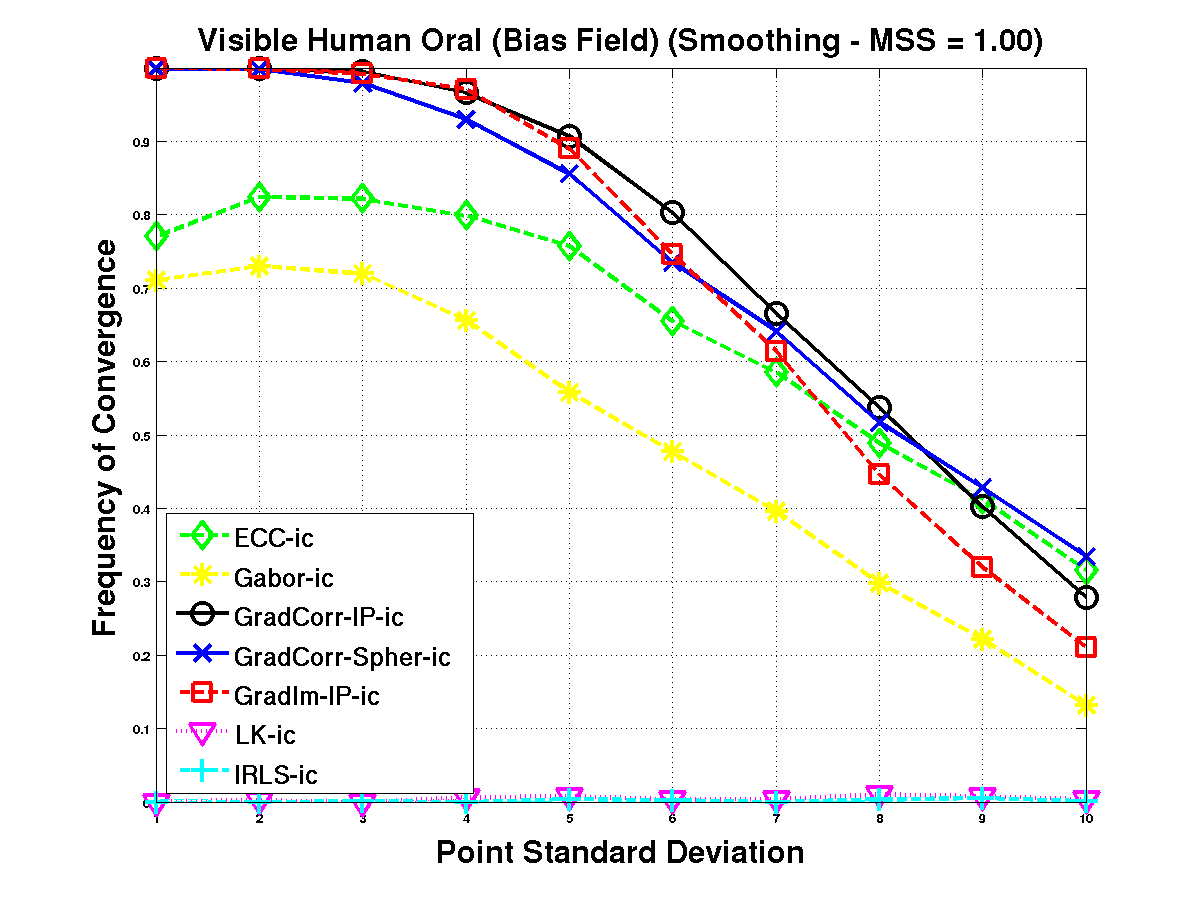
\includegraphics[width=\textwidth]{images/results/biasfield}
                \subcaption{}
                \label{fig:results-biasfield}
        \end{subfigure}
        \begin{subfigure}{0.3\textwidth}
                \centering
                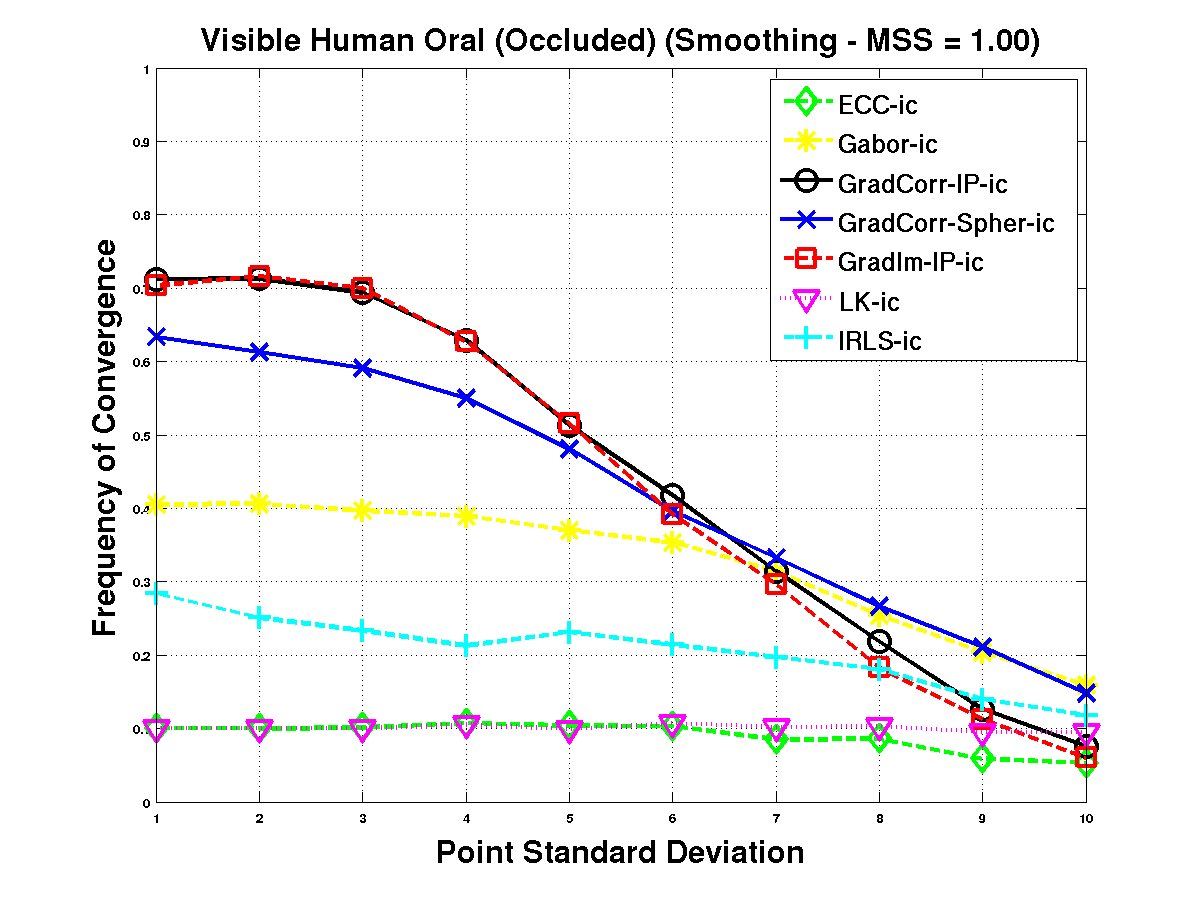
\includegraphics[width=\textwidth]{images/results/occlusion}
                \subcaption{}
                \label{fig:results-occlusion}
        \end{subfigure}
        \begin{subfigure}{0.3\textwidth}
                \centering
                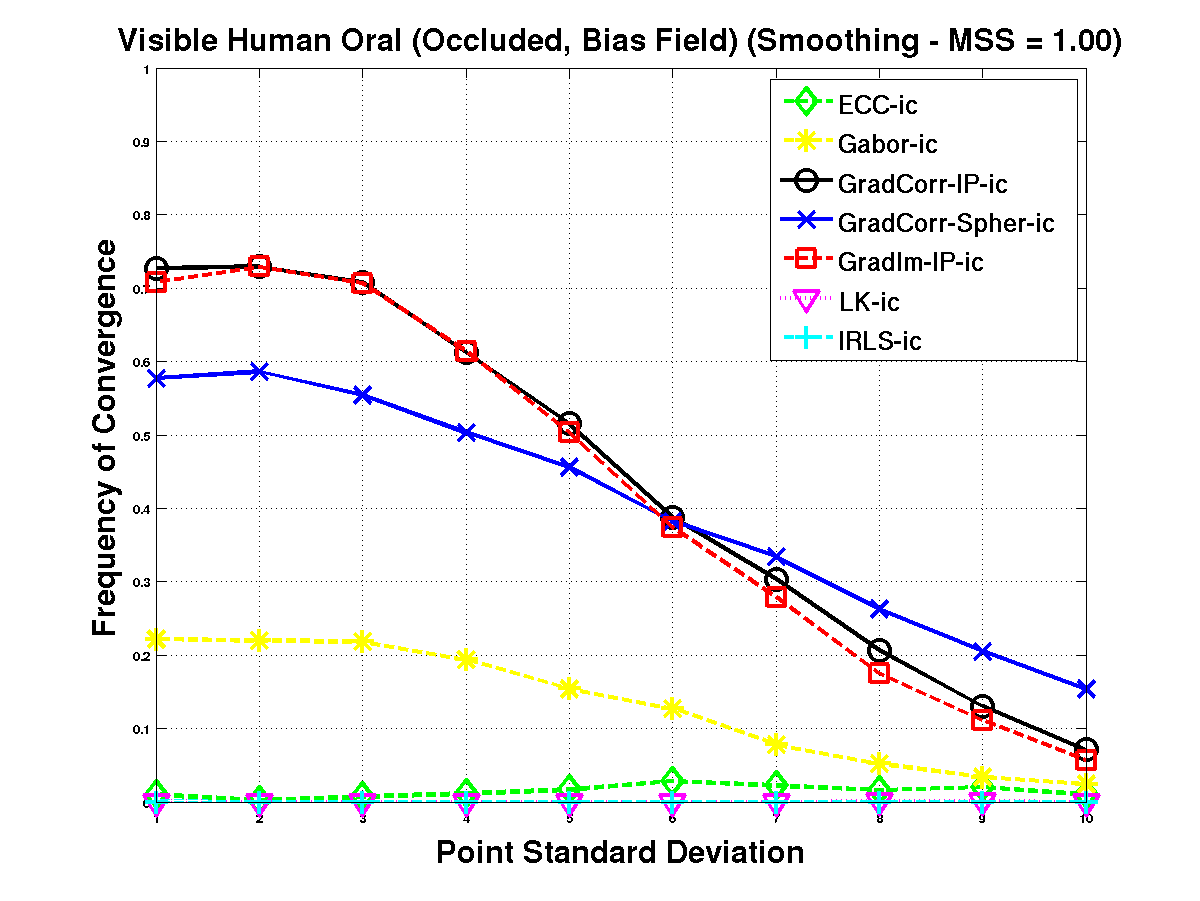
\includegraphics[width=\textwidth]{images/results/occlusion-biasfield}
                \subcaption{}
                \label{fig:results-occlusion-biasfield}
        \end{subfigure}
        \caption{Average frequency of convergence vs Point standard deviation for Visible Human data set. (a) Simulated bias field (b) Occlusions (c) Occlusions + bias field. ECC-ic: green-$\diamond$. Gabor-ic: yellow-*. GradCorr-IP-ic: black-o. GradCorr-Spher-ic: blue-x. GradIm-IP-ic: red-$\square$. LK-ic: magenta-$\bigtriangledown$. IRLS-ic: cyan-+}
        \label{fig:results-corrupted}
\end{figure*}
%%%%%%%%%%%%%%%%%%%%%%%%%%%%%%%%%%%%%%%%%%%%%%%%%%%%%%%%%%%%%%%%%%%%%%%%%%%%%%%%
We measure the performance of our algorithms within an extension of the evaluation framework proposed in \cite{RefWorks:10}. We used the Oral section from the Visible Human data set \cite{RefWorks:81} as the target area. We selected 10 different regions of interest and perturbed the points using Gaussian noise of standard deviation $\sigma$. Using the affine warp defined between the original and perturbed points, we generate a distorted image. Then, given a warp estimate, we compute the new template points and calculate the RMS error between the estimated and correct locations. The performance metric used to assess the algorithms is the average convergence rate for each fixed $\sigma = [1, 10]$, over each of the 10 regions of interest. An algorithm was considered to have converged if it had a final RMS point error of less than $n_1$ pixels after 30 iterations. For each template, 100 convergence tests were performed. Each image was smoothed using Gaussian smoothing before the calculation of derivatives.
%%%%%%%%%%%%%%%%%%%%%%%%%%%%%%%%%%%%%%%%%%%%%%%%%%%%%%%%%%%%%%%%%%%%%%%%%%%%%%%%
\begin{figure}[h]
    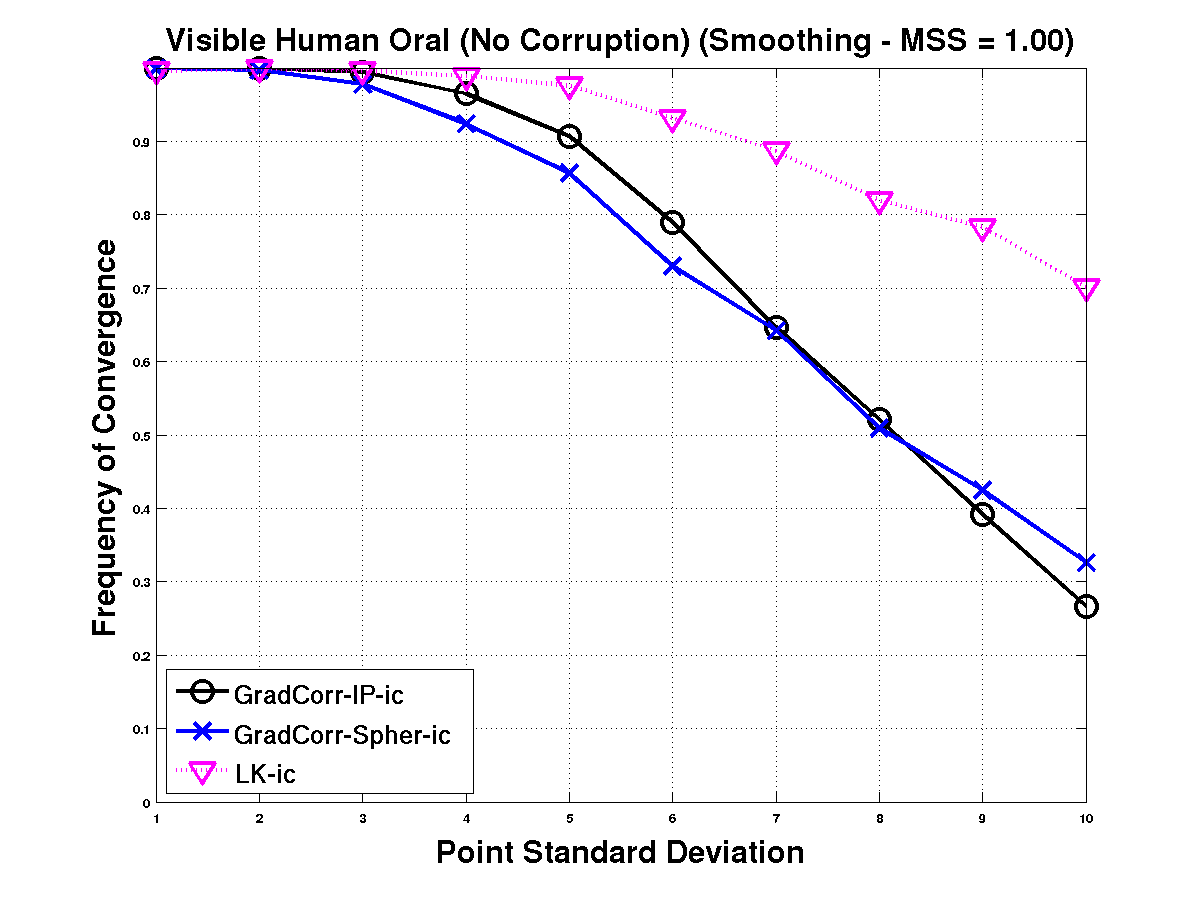
\includegraphics[width=0.45\textwidth]{images/results/nocorruption}
    \caption{Average frequency of convergence vs Point standard deviation for Visible Human data set with no corruption to the images. GradCorr-IP-ic: black-o. GradCorr-Spher-ic: blue-x. LK-ic: magenta-$\bigtriangledown$.}
    \label{fig:results-nocorruption}
\end{figure}
%%%%%%%%%%%%%%%%%%%%%%%%%%%%%%%%%%%%%%%%%%%%%%%%%%%%%%%%%%%%%%%%%%%%%%%%%%%%%%%%

%%%%%%%%%%%%%%%%%%%%%%%%%%%%%%%%%%%%%%%%%%%%%%%%%%%%%%%%%%%%%%%%%%%%%%%%%%%%%%%%
\subsection{Experiments Without Corruption}\label{subsec:results-nocorruption}
%%%%%%%%%%%%%%%%%%%%%%%%%%%%%%%%%%%%%%%%%%%%%%%%%%%%%%%%%%%%%%%%%%%%%%%%%%%%%%%%
In this subsection, we present our performance evaluation results obtained without applying any corruption to the 3D images. We considered alignments with errors of less than $n_1 = 1.0$ to have converged. We compared the performance of the inverse-compositional LK algorithm (LK-ic) with both forms of our algorithm, (GradCorr-IP-IC) and (GradCorr-Sph-IC). 

As Figure~\ref{fig:results-nocorruption} shows, the LK algorithm outperforms both of the proposed methods for this experiment. This result was in line with our expectations, as the distorted image is generated directly from the original image without any outliers. Since both of our proposed methods discard information in the form of the gradient magnitude, they inevitably perform worse than the LK algorithm. However, the difference between our two algorithms is negligible, which is expected given that they both discard the same amount of information.
%%%%%%%%%%%%%%%%%%%%%%%%%%%%%%%%%%%%%%%%%%%%%%%%%%%%%%%%%%%%%%%%%%%%%%%%%%%%%%%%
\subsection{Experiments With Corruption}\label{subsec:results-corrupted}
%%%%%%%%%%%%%%%%%%%%%%%%%%%%%%%%%%%%%%%%%%%%%%%%%%%%%%%%%%%%%%%%%%%%%%%%%%%%%%%%
In this subsection, we present three separate experiments: images with a simulated bias field, an occlusion and an occlusion + a simulated bias field. We include the performance of both of our algorithms (GradCorr-IP-IC) and (GradCorr-Sph-IC), as well as implementations of four other 2D alignment algorithms extended into 3D. The four algorithms we compared with are: the inverse-compositional LK algorithm (LK-ic) \cite{RefWorks:10}, the enhanced correlation coefficient algorithm (ECC-ic) \cite{RefWorks:59}, the iteratively re-weighted least squares algorithm (IRLS-ic) \cite{RefWorks:53} and the Gabor-Fourier LK algorithm (Gabor-ic) \cite{RefWorks:73}. We also include a variant of our algorithm that does not separate orientation and intensity. This algorithm, which we call (GradIm-IP-ic), uses the inner product relationship, but does not differentiate between intensities and gradients. This algorithm illustrates the performance improvement gained by solving a problem that accounts for the relationship between orientation and intensity.

Bias fields were simulated by multiplying an image region by a weighted filter that linearly interpolates between $1$ in the top-left of the image to $0.001$ in the bottom right. Each bias field was applied from left-to-right (x-y plane) across a slice (z-plane) in the 3D image, as shown in Figure~\ref{fig:biasfield-example}. Occluded sections were created synthetically by randomly placing image sections taken from the white matter area of the brain, and putting them into every slice of the 3D image, as shown in Figure~\ref{fig:occlusion-example}.
%%%%%%%%%%%%%%%%%%%%%%%%%%%%%%%%%%%%%%%%%%%%%%%%%%%%%%%%%%%%%%%%%%%%%%%%%%%%%%%%
\begin{figure}[b]
        \centering
        \begin{subfigure}{0.22\textwidth}
                \centering
                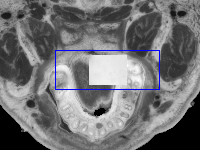
\includegraphics[width=\textwidth]{images/occluded-example}
                \subcaption{}
                \label{fig:occlusion-example}
        \end{subfigure}
        \begin{subfigure}{0.22\textwidth}
                \centering
                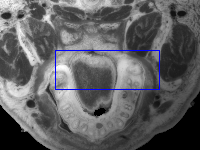
\includegraphics[width=\textwidth]{images/biasfield-example}
                \subcaption{}
                \label{fig:biasfield-example}
        \end{subfigure}
        \caption{(a) Example of an occluded slice of the 3D volume. (b) Example of a slice with a bias field applied to it. In both images the blue rectangle represents the template area being considered.}
        \label{fig:affine-examples}
\end{figure}
%%%%%%%%%%%%%%%%%%%%%%%%%%%%%%%%%%%%%%%%%%%%%%%%%%%%%%%%%%%%%%%%%%%%%%%%%%%%%%%%

Figure~\ref{fig:results-biasfield} shows that our proposed techniques outperform the state-of-the-art for bias field corruption. The non-robust methods of LK-ic and IRLS-ic are not able to cope with the intensity variation caused by the bias field. Gabor-ic copes reasonably well with this type of corruption due to the illumination invariant properties described in \cite{RefWorks:73}. ECC-ic also copes well, as the enhanced correlation coefficient performs a normalisation of the image pixels, which reduces the effect of the bias field. For larger values of $\sigma$, GradCorr-IP-IC outperforms GradIm-IP-IC by almost 10\%. This shows the benefit of considering both orientation as well as intensity for aligning images corrupted with a bias field.

Figure~\ref{fig:results-occlusion} shows that our proposed techniques are also very robust to occlusions. IRLS-ic performs better under these situations as it is able to discard some of the outliers that bias the alignment. The normalisation step in ECC-ic has no benefit in suppressing this sort of bias, and so it performs very similarly to the non-robust LK-ic algorithm.

Finally, in Figure~\ref{fig:results-occlusion-biasfield} we see that even under occlusion and illumination change, our proposed techniques perform impressively. Other than our techniques, only Gabor-ic is able to make any attempt at aligning the images, and even then only in 22\% of attempts. This is due to the illumination invariant properties of Gabor-ic described earlier.
%\section{Conclusion}\label{sec:conclusion}
We introduced a kernel-based framework for performing component analysis of normals. We linked existing projection methods, the azimuthal equidistant projection and principal geodesic analysis, to a unified framework. We show that, with the help of our kernel-based formulation, component analysis can be performed directly upon normals without transformation. We also propose a new robust kernel for performing component analysis on normals. In particular, our new kernel based on the angular distance, shows qualitative and quantitative improvement over existing techniques in both artificial reconstruction and SFS settings.

% if have a single appendix:
%\appendix[Proof of the Zonklar Equations]
% or
%\appendix  % for no appendix heading
% do not use \section anymore after \appendix, only \section*
% is possibly needed

% use appendices with more than one appendix
% then use \section to start each appendix
% you must declare a \section before using any
% \subsection or using \label (\appendices by itself
% starts a section numbered zero.)


%\appendices
\section{LK derivations}
In this section we give a detailed derivation on how Equation~\ref{eq:cosine-inner-product} can be optimised, as introduced in Section~\ref{subsec:lk-inner-product}.

The motion parameters, $\p$, can be estimated by maximising
%%%%%%%%%%%%%%%%%%%%%%%%%%%%%%%%%%%%%%%%%%%%%%%%%%%%%%%%%%%%%%%%%%%%%%%%%%%%%%%%
\begin{equation}
  \begin{aligned}\label{eq:eucq}
    q &= \sum \limits_{k \in P} \cos [\phi (k)] \\
      &= \sum \limits_{k \in P} \tildeg_{1,x}(k)\tildeg_{2,x}(k) + \tildeg_{1,y}(k)\tildeg_{2,y}(k) + \tildeg_{1,z}(k)\tildeg_{2,z}(k)
  \end{aligned}
\end{equation}
%%%%%%%%%%%%%%%%%%%%%%%%%%%%%%%%%%%%%%%%%%%%%%%%%%%%%%%%%%%%%%%%%%%%%%%%%%%%%%%%
However, a first order Taylor expansion of either $\tildeg_1$ or $\tildeg_2$ with respect to $\deltap$ results in a linear function of $\deltap$. In order to avoid the computation of the second order Taylor expansion, we take the approach outlined by \cite{RefWorks:59} and normalise the cost function according to $\tildeg_2$. This yields a cost function of the form
%%%%%%%%%%%%%%%%%%%%%%%%%%%%%%%%%%%%%%%%%%%%%%%%%%%%%%%%%%%%%%%%%%%%%%%%%%%%%%%%
\begin{equation}
  \begin{aligned}\label{eq:eucqg2}
    q &= \frac{\sum \limits_{k \in P} \tildeg_{1,x}(k)\tildeg_{2,x}(k) + \tildeg_{1,y}(k)\tildeg_{2,y}(k) + \tildeg_{1,z}(k)\tildeg_{2,z}(k)}{\sqrt{\sum \limits_{k \in P} \tildeg_{2,x}^2(k) + \tildeg_{2,y}^2(k) + \tildeg_{2,z}^2(k)}} \\
      &= \frac{\tildeg_{1,x}^T \tildeg_{2,x} + \tildeg_{1,y}^T \tildeg_{2,y} + \tildeg_{1,z}^T \tildeg_{2,z}}{\sqrt{\tildeg_{2,x}^T \tildeg_{2,x} + \tildeg_{2,y}^T \tildeg_{2,y} + \tildeg_{2,z}^T \tildeg_{2,z}}}
  \end{aligned}
\end{equation}
%%%%%%%%%%%%%%%%%%%%%%%%%%%%%%%%%%%%%%%%%%%%%%%%%%%%%%%%%%%%%%%%%%%%%%%%%%%%%%%%
where, if we linearize $\tildeg_2$, we have a non-linear function of $\deltap$. We can then maximise $q$ with respect to $\p$ by assuming a current estimate of $\p$ is known and looking for an increment $\deltap$ that maximises (\ref{eq:eucqg2}).
%%%%%%%%%%%%%%%%%%%%%%%%%%%%%%%%%%%%%%%%%%%%%%%%%%%%%%%%%%%%%%%%%%%%%%%%%%%%%%%%
\subsection{The inner product inverse-compositional gradient correlation algorithm}\label{subsec:3deucinvcomp}
We choose to provide the derivation of the inverse-compositional form of the algorithm, due to the pre-computable nature of the Hessian in this form. However, a forward-additive version of the algorithm would be simple to implement following a similar logic.

For the inverse-compositional algorithm, we swap the roles of $\I_1$ and $\I_2$ and the cost function is defined as
%%%%%%%%%%%%%%%%%%%%%%%%%%%%%%%%%%%%%%%%%%%%%%%%%%%%%%%%%%%%%%%%%%%%%%%%%%%%%%%%
% WITH NOTATION
%\begin{equation}\label{eq:eucinvcomp}
%    q = \frac{(\tildeg_{2,x}[p])^T (\tildeg_{1,x}[\deltap])+ (\tildeg_{2,y}[p])^T (\tildeg_{1,y}[\deltap]) + (\tildeg_{2,z}[p])^T (\tildeg_{1,z}[\deltap])}{\sqrt{(\tildeg_{1,x}[\deltap])^T (\tildeg_{1,x}[\deltap]) +(\tildeg_{1,y}[\deltap])^T (\tildeg_{1,y}[\deltap]) + (\tildeg_{1,z}[\deltap])^T (\tildeg_{1,z}[\deltap])}}
%\end{equation}
%%%%%%%%%%%%%%%%%%%%%%%%%%%%%%%%%%%%%%%%%%%%%%%%%%%%%%%%%%%%%%%%%%%%%%%%%%%%%%%%%
%%%%%%%%%%%%%%%%%%%%%%%%%%%%%%%%%%%%%%%%%%%%%%%%%%%%%%%%%%%%%%%%%%%%%%%%%%%%%%%%
\begin{equation}\label{eq:eucinvcomp}
    q = \frac{\tildeg_{2,x}^T \tildeg_{1,x} + \tildeg_{2,y}^T \tildeg_{1,y} + \tildeg_{2,z}^T \tildeg_{1,z}}{\sqrt{\tildeg_{1,x}^T \tildeg_{1,x} + \tildeg_{1,y}^T \tildeg_{1,y} + \tildeg_{1,z}^T \tildeg_{1,z})}}
\end{equation}
%%%%%%%%%%%%%%%%%%%%%%%%%%%%%%%%%%%%%%%%%%%%%%%%%%%%%%%%%%%%%%%%%%%%%%%%%%%%%%%%%
where $\tildeg_1$ has a dependency on $\deltap$ and $\tildeg_2$ has a dependency on $\p$, which have been omitted for notational simplicity.

$\I_2$ is then updated at each iteration using the compositional update $\W(\x;\p) \leftarrow \W(\x;\p) \circ (\W(\x;\p))^{-1}$. It is also assumed that $\W(\x;\zero) = \x$ and thus the Taylor expansion is performed around zero. The derivation is split in to separate entities for each dimension, $x$, $y$ and $z$. The first Taylor expansion on $\tildeg_{1,x}[\p + \deltap]$ produces
%%%%%%%%%%%%%%%%%%%%%%%%%%%%%%%%%%%%%%%%%%%%%%%%%%%%%%%%%%%%%%%%%%%%%%%%%%%%%%%%
\begin{equation}\label{eq:eucgx}
    \tildeg_{1,x}[\deltap] \approx \tildeg_{1,x}[\zero] + \nabla \tildeg_{1,x}[\zero] \deltap
\end{equation}
%%%%%%%%%%%%%%%%%%%%%%%%%%%%%%%%%%%%%%%%%%%%%%%%%%%%%%%%%%%%%%%%%%%%%%%%%%%%%%%%
By the chain rule we can decompose $\nabla \tildeg_{1,x}[\zero]$ in to
%%%%%%%%%%%%%%%%%%%%%%%%%%%%%%%%%%%%%%%%%%%%%%%%%%%%%%%%%%%%%%%%%%%%%%%%%%%%%%%%
\begin{equation}
  \begin{aligned}\label{eq:nablagx}
    \nabla \tildeg_{1,x}[\zero] &= \frac{\partial \tildeg_{1,x}[\p]}{\partial \p}\Big|_{p=0} \\
                              &= \frac{\partial f(\g_{1,x}[\p])}{\partial \g_{1,x}[\p]} \; \frac{\partial \g_{1,x}[\p]}{\partial \p}\Big|_{\p=0}
  \end{aligned}
\end{equation}
%%%%%%%%%%%%%%%%%%%%%%%%%%%%%%%%%%%%%%%%%%%%%%%%%%%%%%%%%%%%%%%%%%%%%%%%%%%%%%%%
We provide the derivation for (\ref{eq:nablagx}) as follows:
%%%%%%%%%%%%%%%%%%%%%%%%%%%%%%%%%%%%%%%%%%%%%%%%%%%%%%%%%%%%%%%%%%%%%%%%%%%%%%%%
\begin{equation}
  \begin{aligned}\label{eq:derivefgx}
    \frac{\partial f(\g_{1,x}[\p])}{\partial \g_{1,x}[\p]}\Big|_{\p=0} &= \frac{\partial \frac{\g_{1,x}[\p]}{\sqrt{\g_{1,x}^2[\p] + \g_{1,y}^2[\p] + \g_{1,z}^2[\p]}}}{\partial \g_{1,x}[\p]}\Bigg|_{\p=0} \\
     &= \frac{\g_{1,y}^2[\zero] + \g_{1,z}[\zero]^2}{(\g_{1,x}^2[\zero] + \g_{1,y}^2[\zero] + \g_{1,z}^2[\zero])^{3/2}}
  \end{aligned}
\end{equation}
%%%%%%%%%%%%%%%%%%%%%%%%%%%%%%%%%%%%%%%%%%%%%%%%%%%%%%%%%%%%%%%%%%%%%%%%%%%%%%%%
%%%%%%%%%%%%%%%%%%%%%%%%%%%%%%%%%%%%%%%%%%%%%%%%%%%%%%%%%%%%%%%%%%%%%%%%%%%%%%%%
\begin{equation}\label{eq:derivegxp}
    \frac{\partial \g_{1,x}[\p]}{\partial \p}\Big|_{\p=0} = [ \g_{1,xx}[\zero](k) \; \g_{1,xy}[\zero](k) \; \g_{1,xz}[\zero](k) ] \frac{\partial \W}{\partial \p}
\end{equation}
%%%%%%%%%%%%%%%%%%%%%%%%%%%%%%%%%%%%%%%%%%%%%%%%%%%%%%%%%%%%%%%%%%%%%%%%%%%%%%%%%
Where the result from (\ref{eq:derivegxp}) is as described by Equation (12) of \cite{RefWorks:6}. To simplify the expressions, we define a function $f(a,b)$, such that
%%%%%%%%%%%%%%%%%%%%%%%%%%%%%%%%%%%%%%%%%%%%%%%%%%%%%%%%%%%%%%%%%%%%%%%%%%%%%%%%
\begin{equation}\label{eq:f-simplify}
    f(a,b) = \frac{\g_{1,a}^2 + \g_{1,b}^2}{(\g_{1,x}^2 + \g_{1,y}^2 + \g_{1,z}^2)^{3/2}}
\end{equation}
%%%%%%%%%%%%%%%%%%%%%%%%%%%%%%%%%%%%%%%%%%%%%%%%%%%%%%%%%%%%%%%%%%%%%%%%%%%%%%%%%
Therefore, we define $\tildeg_{1,x}[\deltap]$, $\tildeg_{1,y}[\deltap]$ and $\tildeg_{1,z}[\deltap]$ as
%%%%%%%%%%%%%%%%%%%%%%%%%%%%%%%%%%%%%%%%%%%%%%%%%%%%%%%%%%%%%%%%%%%%%%%%%%%%%%%%
\begin{equation}
  \begin{aligned}\label{eq:eucgyz}
    \tildeg_{1,x}[\deltap] &\approx \tildeg_{1,x}[\zero] + f(y,z)[\zero] \; \nabla \g_{1,x}[\zero] \frac{\partial \W}{\partial \p} \deltap \\  
    \tildeg_{1,y}[\deltap] &\approx \tildeg_{1,y}[\zero] + f(x,z)[\zero] \; \nabla \g_{1,y}[\zero] \frac{\partial \W}{\partial \p} \deltap \\
    \tildeg_{1,z}[\deltap] &\approx \tildeg_{1,z}[\zero] + f(x,y)[\zero] \; \nabla \g_{1,z}[\zero] \frac{\partial \W}{\partial \p} \deltap
  \end{aligned}
\end{equation}
%%%%%%%%%%%%%%%%%%%%%%%%%%%%%%%%%%%%%%%%%%%%%%%%%%%%%%%%%%%%%%%%%%%%%%%%%%%%%%%%
 and
%%%%%%%%%%%%%%%%%%%%%%%%%%%%%%%%%%%%%%%%%%%%%%%%%%%%%%%%%%%%%%%%%%%%%%%%%%%%%%%%
\begin{equation}
  \begin{aligned}\label{eq:euc-second-order-derivs}
    \nabla \g_{1,x}[\zero] &= [ \g_{1,xx}[\zero](k) \; \g_{1,xy}[\zero](k) \; \g_{1,xz}[\zero](k) ] \\
    \nabla \g_{1,y}[\zero] &= [ \g_{1,yx}[\zero](k) \; \g_{1,yy}[\zero](k) \; \g_{1,yz}[\zero](k) ] \\
    \nabla \g_{1,z}[\zero] &= [ \g_{1,zx}[\zero](k) \; \g_{1,zy}[\zero](k) \; \g_{1,zz}[\zero](k) ]
  \end{aligned}
\end{equation}
%%%%%%%%%%%%%%%%%%%%%%%%%%%%%%%%%%%%%%%%%%%%%%%%%%%%%%%%%%%%%%%%%%%%%%%%%%%%%%%%

Equations (\ref{eq:eucgyz}) and (\ref{eq:eucgx}) can be plugged in to (\ref{eq:eucqg2}) to arrive at the cost function $q(\deltap)$. In the formulae below, the dependencies on $[\zero]$ and $[\deltap]$ are dropped for notational simplicity. The numerator is as follows
%%%%%%%%%%%%%%%%%%%%%%%%%%%%%%%%%%%%%%%%%%%%%%%%%%%%%%%%%%%%%%%%%%%%%%%%%%%%%%%%
\begin{equation}
  \begin{aligned}\label{eq:q_dp_num}
    q(\deltap) &= \tildeg_{2,x}^T (\tildeg_{1,x} + \nabla \tildeg_{1,x} \deltap) + \tildeg_{2,y}^T (\tildeg_{1,y} + \nabla \tildeg_{1,y} \deltap) \\
    & \hspace{4 mm} + \tildeg_{2,z}^T (\tildeg_{1,z} + \nabla \tildeg_{1,z} \deltap) \\
    &= \tildeg_{2,x}^T \tildeg_{1,x} + \tildeg_{2,y}^T \tildeg_{1,y} + \tildeg_{2,z}^T \tildeg_{1,z} \\     
    & \hspace{4 mm} + \left( \tildeg_{2,x}^T \nabla \tildeg_{1,x} + \tildeg_{2,y}^T \nabla \tildeg_{1,y} + \tildeg_{2,z}^T \nabla \tildeg_{1,z} \right) \deltap \\
    %&= [\tildeg_{2,x} \; \tildeg_{2,y} \; \tildeg_{2,z}]^T [\tildeg_{1,x} \; \tildeg_{1,y} \; \tildeg_{1,z}] + [\tildeg_{2,x} \; \tildeg_{2,y} \; \tildeg_{2,z}]^T [\nabla \tildeg_{1,x} \; \nabla \tildeg_{1,y} \; \nabla \tildeg_{1,z}] \deltap \\
    &= q_p + \GTwo^T \J \deltap
  \end{aligned}
\end{equation}
%%%%%%%%%%%%%%%%%%%%%%%%%%%%%%%%%%%%%%%%%%%%%%%%%%%%%%%%%%%%%%%%%%%%%%%%%%%%%%%%
where $\J = \left[ \nabla \tildeg_{2,x} \; \nabla \tildeg_{2,y} \; \nabla \tildeg_{2,z} \right]^T$ as described in (\ref{eq:nablagx})-(\ref{eq:derivegxp}) and $\GTwo = \left[ \tildeg_{2,x} \; \tildeg_{2,y} \; \tildeg_{2,z} \right]^T$. The denominator is defined as
\begin{equation}
  \begin{aligned}\label{eq:q_dp_denom}
    q(\deltap) &= \left( (\tildeg_{1,x} + \nabla \tildeg_{1,x} \deltap)^T (\tildeg_{1,x} + \nabla \tildeg_{1,x} \deltap) + \right. \\
    & \hspace{6 mm} \left. (\tildeg_{1,y} + \nabla \tildeg_{1,y} \deltap)^T (\tildeg_{1,y} + \nabla \tildeg_{1,y} \deltap) + \right. \\
    & \hspace{5 mm} \left. (\tildeg_{1,z} + \nabla \tildeg_{1,z} \deltap)^T (\tildeg_{1,z} + \nabla \tildeg_{1,z} \deltap) \right)^{1/2} \\
    %&= \left( \sum_k (\tildeg_{1,x} + \nabla \tildeg_{1,x} \deltap)^2 + (\tildeg_{1,y} + \nabla \tildeg_{1,y} \deltap)^2 + \\
    %& \hspace{12 mm} (\tildeg_{1,z} + \nabla \tildeg_{1,z} \deltap)^2 \right)^{1/2} \\
    &= \left( \sum_k \tildeg^2_{1,x} + \tildeg^2_{1,y} + \tildeg^2_{1,z} + 2 \; \tildeg_{1,x} \nabla \tildeg_{1,x} \deltap + \right. \\
    & \hspace{4 mm} \left. 2 \; \tildeg_{1,y} \nabla \tildeg_{1,y} \deltap + 2 \; \tildeg_{1,z} \nabla \tildeg_{1,z} \deltap + \right. \\
    & \hspace{4 mm} \left. \vphantom{\sum_k} (\nabla \tildeg_{1,x} \deltap)^2 + (\nabla \tildeg_{1,y} \deltap)^2 +(\nabla \tildeg_{1,z} \deltap)^2 \right)^{1/2} \\
    &= \sqrt{\norm{\GOne}^2 + 2 \GOne^T \J \deltap + \deltap^T \J^T \J \deltap}
  \end{aligned}
\end{equation}
%%%%%%%%%%%%%%%%%%%%%%%%%%%%%%%%%%%%%%%%%%%%%%%%%%%%%%%%%%%%%%%%%%%%%%%%%%%%%%%%
We can then combine (\ref{eq:q_dp_num}) and (\ref{eq:q_dp_denom}) together to form the cost function
%%%%%%%%%%%%%%%%%%%%%%%%%%%%%%%%%%%%%%%%%%%%%%%%%%%%%%%%%%%%%%%%%%%%%%%%%%%%%%%%
\begin{equation}\label{eq:q_dp}
    q(\deltap) = \frac{q_p + \GTwo^T \J \deltap}{\sqrt{\norm{\GOne}^2 + 2 \GOne^T \J \deltap + \deltap^T \J^T \J \deltap}}
\end{equation}
%%%%%%%%%%%%%%%%%%%%%%%%%%%%%%%%%%%%%%%%%%%%%%%%%%%%%%%%%%%%%%%%%%%%%%%%%%%%%%%%
where $\GOne = \left[ \tildeg_{1,x} \; \tildeg_{1,y} \; \tildeg_{1,z} \right]^T$. Finally, we maximise (\ref{eq:q_dp}) as in \cite{RefWorks:59} We first note that we have a cost function of the form
%%%%%%%%%%%%%%%%%%%%%%%%%%%%%%%%%%%%%%%%%%%%%%%%%%%%%%%%%%%%%%%%%%%%%%%%%%%%%%%%
\begin{equation*}
    f(x) = \frac{u + \boldsymbol{u}\boldsymbol{x}}{\sqrt{v + 2 \boldsymbol{v}^T \boldsymbol{x} + \boldsymbol{x}^T  \boldsymbol{Q} \boldsymbol{x}}}
\end{equation*}
%%%%%%%%%%%%%%%%%%%%%%%%%%%%%%%%%%%%%%%%%%%%%%%%%%%%%%%%%%%%%%%%%%%%%%%%%%%%%%%%
and we can therefore derive two different maxima. 

\textbf{(Case 1)} $u > \boldsymbol{u}^T \boldsymbol{Q}^{-1} \boldsymbol{v}$: Here we have a maximum of $x$ which is attainable from the equation
%%%%%%%%%%%%%%%%%%%%%%%%%%%%%%%%%%%%%%%%%%%%%%%%%%%%%%%%%%%%%%%%%%%%%%%%%%%%%%%%
\begin{equation}\label{eq:case1}
    x = \boldsymbol{Q}^{-1} \left( \frac{v - \boldsymbol{v}^T  \boldsymbol{Q}^{-1} \boldsymbol{v}}{u - \boldsymbol{u}^T \boldsymbol{Q}^{-1} \boldsymbol{v}} \boldsymbol{u} - \boldsymbol{v} \right)
\end{equation}
%%%%%%%%%%%%%%%%%%%%%%%%%%%%%%%%%%%%%%%%%%%%%%%%%%%%%%%%%%%%%%%%%%%%%%%%%%%%%%%%
\textbf{(Case 2)} $u \le \boldsymbol{u}^T \boldsymbol{Q}^{-1} \boldsymbol{v}$ : Here we have a maximum of $x$ which is attainable from the equation
%%%%%%%%%%%%%%%%%%%%%%%%%%%%%%%%%%%%%%%%%%%%%%%%%%%%%%%%%%%%%%%%%%%%%%%%%%%%%%%%
\begin{equation}\label{eq:case2}
    x = \boldsymbol{Q}^{-1} \left( \lambda \boldsymbol{u} - \boldsymbol{v} \right)
\end{equation}
%%%%%%%%%%%%%%%%%%%%%%%%%%%%%%%%%%%%%%%%%%%%%%%%%%%%%%%%%%%%%%%%%%%%%%%%%%%%%%%%
where $\lambda$ can have the possible values of
%%%%%%%%%%%%%%%%%%%%%%%%%%%%%%%%%%%%%%%%%%%%%%%%%%%%%%%%%%%%%%%%%%%%%%%%%%%%%%%%
\begin{equation}\label{eq:lambda}
    \lambda_1 = \sqrt{\frac{\boldsymbol{v}^T \boldsymbol{Q}^{-1} \boldsymbol{v}}{\boldsymbol{u}^T \boldsymbol{Q}^{-1} \boldsymbol{u}}} \qquad \lambda_2 = \frac{\boldsymbol{u}^T \boldsymbol{Q}^{-1} \boldsymbol{v} - \boldsymbol{u}^T \boldsymbol{v}}{\boldsymbol{u}^T \boldsymbol{Q}^{-1} \boldsymbol{u}}
\end{equation}
%%%%%%%%%%%%%%%%%%%%%%%%%%%%%%%%%%%%%%%%%%%%%%%%%%%%%%%%%%%%%%%%%%%%%%%%%%%%%%%%
Equation~(\ref{eq:case2}) should only be used when the denominator is negative and thus we are not close to the optimum solution. In this case we are unlikely to ever reach the optimum value and so we choose to use Equation~(\ref{eq:case1}) to calculate our maximum. Through matching of terms between (\ref{eq:case1}) and (\ref{eq:q_dp}) we arrive at
%%%%%%%%%%%%%%%%%%%%%%%%%%%%%%%%%%%%%%%%%%%%%%%%%%%%%%%%%%%%%%%%%%%%%%%%%%%%%%%%
\begin{equation}\label{eq:max_deltap}
    \deltap = (\J^T \J)^{-1} \J^T \left( \frac{\norm{\GOne}^2 - \GOne^T \boldsymbol{P_G} \GOne}{\GTwo^T \GOne - \GTwo^T \boldsymbol{P_G} \GOne} \GTwo - \GOne \right)
\end{equation}
%%%%%%%%%%%%%%%%%%%%%%%%%%%%%%%%%%%%%%%%%%%%%%%%%%%%%%%%%%%%%%%%%%%%%%%%%%%%%%%%
where $\boldsymbol{P_G} \triangleq \J (\J^T \J)^{-1} \J^T$ and $\boldsymbol{P_G}$ is an orthogonal projection operator.

{\small
\bibliographystyle{ieeetr}
\bibliography{egbib}
}

\end{document}
